\chapter{\texorpdfstring{$^{39}\mathrm{\textbf{K}}(\MakeLowercase{p},\gamma)^{40}\mathrm{\textbf{C\MakeLowercase{a}}}$}{39K(p,g)40Ca} Constraints for Globular Cluster NGC 2419}
\label{ch:GC}

%%%%%%%%%%%%%%%%%%%%%%%%%%%%%%%%%%%%%%%%%%%%%%%%%%%%%%%%%%%%%%%%%%%%%%%%%%%%%%%%%%%%%%%%%%%%%
\section{Introduction}

% Globular clusters and anticorrelations in general (See Gratton et al. 2019)
%  3.1) Introduction to globular cluster abundance anticorrelations in general
%  - What is a globular cluster?
%  - Defined by multiple stellar populations (Bedin et al. 2004, Piotto 2007). Show the HR diagram for an example Milky Galaxy
%  - Defined by abundance anticorrelations. Show an example anticorrelation, such as O-Na
%  - Abundance anticorrelations result from pollution/mixing from older stars in the globular cluster (polluter stars) ["The (anti-)correlation among light elements is simply a manifestation of the multiple stellar populations." (Gratton et al. 2019)]
%  - Hydrogen burning in the polluter stars is the mechanism behind these anticorrelations (

This chapter details the original research constraining hydrogen-burning conditions responsible for abundance anomalies in globular clusters. In particular, the observed potassium enrichment and magnesium depletion in red giants of the globular cluster NGC 2419 is reproduced with nuclear reaction network calculations using new nuclear physics information presented in this chapter. A new reaction rate of the key potassium-destroying reaction, $^{39}\mathrm{K}(p,\gamma)^{40}\mathrm{Ca}$, is calculated from the proton partial-widths and resonance energies of astrophysically-important, unbound $^{40}$Ca states measured in the proton-transfer reaction $^{39}\mathrm{K}(^{3}\mathrm{He},d)^{40}\mathrm{Ca}$. The reaction rate is significantly constrained for $T \lesssim 110$ MK. Monte Carlo network calculations will show new temperature-density constraints for hydrogen-burning, compared with that of the previously calculated reaction rate. Hot-bottom burning in Super-AGB stars is investigated as a polluter candidate driving the Mg--K anticorrelation in NGC 2419, as well as other abundance patterns involving potassium.

\section{Globular Clusters}

% From PRL (Before cutting material):
\begin{comment}
The abundance pattern of % (some)? b/c we understand the O-Na and Mg-Al ones pretty well 
globular clusters is still poorly understood, despite evidence of multiple stellar populations within each cluster \cite{Bedin2004,Piotto2007} and abundance anticorrelations of light element pairs between low-mass cluster stars, such as C--N, O--Na, and Mg--Al (see Gratton \emph{et al.} \cite{Gratton2012} for a recent review). The origin of these anticorrelations likely involves the currently observed globular cluster stars forming from the matter of earlier cluster stars, or \emph{polluter stars}, because the low-mass stars in which these anticorrelations have been observed do not produce sufficiently high temperatures to account for changes in abundance of the above elements.
%The origin of these anticorrelations likely involves matter mixing between stellar populations because the low-mass stars in which these anticorrelations have been observed do not produce sufficiently high temperatures to account for changes in abundance of the above elements. The currently observed globular cluster stars must therefore have been formed out of the polluted material from earlier globular cluster stars, or \emph{polluter stars}. 
The O--Na and Mg--Al abundance anticorrelations have been shown to be reproduced by low-temperature hydrogen burning at about 75 MK in the polluter stars of globular cluster NGC 6752 \cite{Prantzos2007}. However, the list of candidate sources for the polluter stars in NGC 6752, and for many other globular clusters, is quite long. % Cite them? 8 according to Iliadis et al. 2016
\end{comment}

Globular clusters are compact conglomerates of stars associated with all types of galaxies. They are typically on the order of 1 pc to a few tens of pc in radius. They are very old, in most cases having an age of about 10 Gyr, and they are also quite luminous, with a mean absolute visual magnitude $M_{V} = -7$. Peak globular cluster formation is thought to pre-date most stellar formation in galaxies, and they may have played a crucial role in early galaxy formation \cite{Gratton2019}. In the Milky Way galaxy, they often have low metallicity and are distributed throughout the halo, the thick disk, and the bulge. These properties, while interesting in their own right, are not what have made globular clusters garner considerable interest in the last few decades.

A characteristic recently attributed to globular clusters, which distinguishes them from similar objects such as open clusters, is the presence of chemical inhomogeneities among their low-mass stars. Once labeled \emph{abundance anomalies}, these inhomogeneities take the form of anticorrelations among the abundances of light element pairs, such as O--Na and Mg--Al. A new definition of globular clusters that includes this characteristic was suggested by Ref. \cite{Carretta2010}, since almost every globular cluster in which abundances have been observed has exhibited an O--Na anticorrelation. 
% ``In (almost) all studied GCs the Na-O anticorrelation has been found. One exception is Terzan 7, where no spread in O abundances has been found in the (only) seven stars observed by Sbordone et al. (2007), and may then be the most massive cluster observed so far without the Na-O anticorrelation. The other one is Pal 12, where Cohen (2004) finds very uniform O and Na abundances, but only for four stars." (Carretta et al. 2010).
% Sbordone, L., Bonifacio, P., Buonanno, R., et al. 2007, A&A, 465, 815
% Cohen, J. G. 2004, AJ, 127, 1545
The only exceptions are Terzan 7 and Pal 12, where the simultaneous Na and O abundances of only 7 \cite{Sbordone2007} and 4 \cite{Cohen2004} stars were observed, respectively. Other anticorrelations and correlations are exhibited in some, but not all globular clusters, making each cluster distinguishable by the combination and extent of their abundance inhomogeneities. These cluster-to-cluster differences are primarily driven by differences in luminosity and metallicity. Meanwhile, no anticorrelations have ever been observed in open clusters \cite{Gratton2019}.

Fig. \ref{fig:O-Na} shows the ubiquitous O--Na anticorrelation in 1,200 red giants among all 19 globular clusters sampled by Ref. \cite{Carretta2010}. The red giants with an enhanced Na abundance are associated with a depletion in O abundance, and vice versa. The populations of red giants are split into 3 categories based on the extent of their Na enrichment, and associated O depletion. These populations are the primordial (P), extreme (E), and intermediate (I) components, as indicated in the first panel of Fig. \ref{fig:O-Na}. The primordial population is Na-poor/O-rich, the extreme population is Na-rich/O-poor, and the intermediate population is in-between. The primordial population is so-called because the same abundance pattern is typical of field stars with a similar metallicity. However, the Na and O abundances of the intermediate and extreme populations indicates that these red giants went through an unknown process. Low-mass stars like red giants and main sequence stars do not reach the high temperatures necessary for the nucleosynthesis chains that produce the observed Na and O abundances. This reasoning also applies to the other observed anticorrelations in globular clusters \cite{Prantzos2007}.

\begin{figure}[t]
\centering
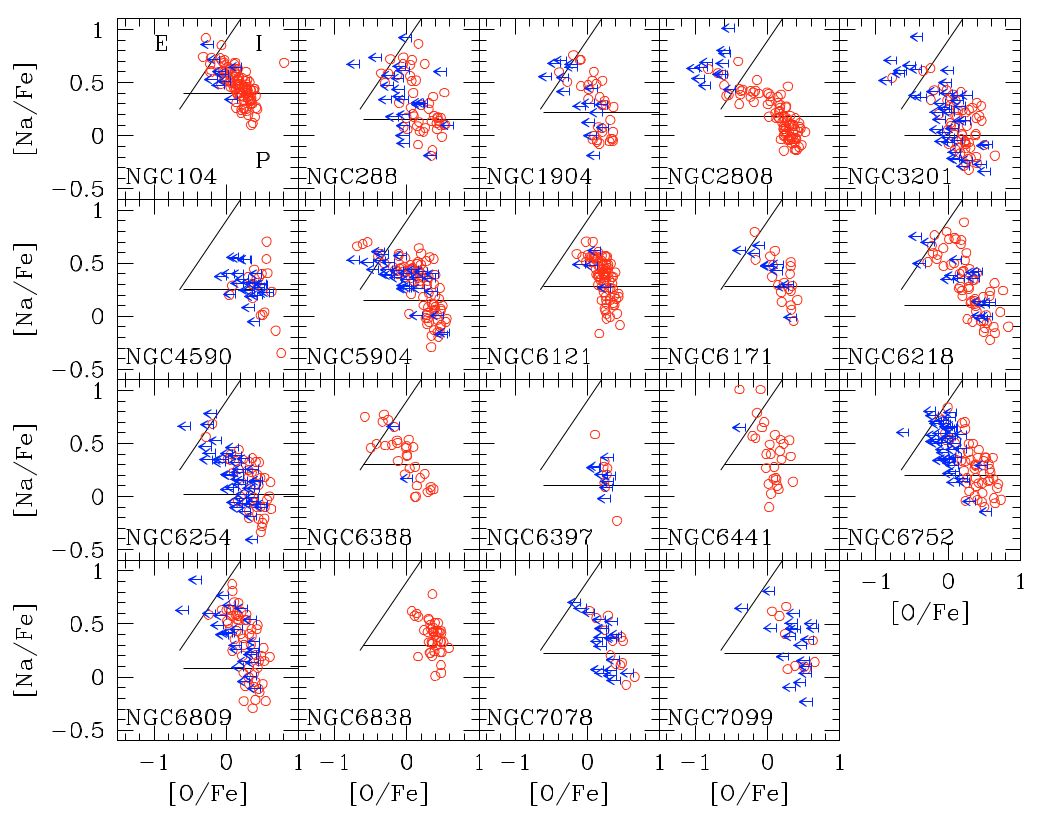
\includegraphics[width=6.5in]{Chapter-6/figs/O-Na.png}
\caption{\label{fig:O-Na}The O--Na anticorrelation of 1,200 red giants among all 19 globular clusters observed in the survey of Ref. \cite{Carretta2010}. Blue arrows indicate upper limits in O abundances, while lines separate different populations of red giants based on their relative O and Na richness. Primordial (P), extreme (E), and intermediate (I) populations are labeled in the first panel. See text for definitions of these populations. Adapted from \cite{Carretta2010}.}
\end{figure}

% PARAGRAPH 1: Cannot be in situ - must be mixing. Evidence for multiple stellar populations - pg 2 of Carretta2010 and Prantzos2007

% ``The (anti-)correlation among light elements is simply a manifestation of the multiple stellar populations." (Gratton et al. 2019) pg 12

% ``The variations are also found among unevolved stars currently on the main sequence (MS) of GCs (Gratton et al. 2001; Ramirez & Cohen 2002; Carretta et al. 2004; D’Orazi et al. 2010). This unequivocally implies that this composition has been imprinted in the gas by a previous generation of stars. The necessity of this conclusion stems from low-mass MS stars not being able to reach the high temperatures for the nucleosynthetic chains required to produce the observed inter-relations between the elements (in particular the Mg-Al anticorrelation). This calls for a class of now extinct stars, more massive than the low-mass ones presently evolving in GCs, as the site for the nucleosynthesis." (Carretta et al. 2010) pg 2

The most likely scenario explaining these inhomogeneities is that the currently observed stars are part of a second generation which formed from the ashes of an older, first generation of stars. The material ejected from these more-massive first generation stars upon their death likely polluted the inter-cluster medium where the second generation stars began to form. Hence, these first generation stars are sometimes called \emph{polluter stars}, a class of massive, extinct stars that are the origin of the apparent abundance anomalies. Different generations of stars exhisting in a given globular cluster would provide evidence for \emph{multiple stellar populations}. This premise has been widely debated over the last few decades, with most research supporting it at present \cite{Gratton2004,Gratton2012,Gratton2019}.

% PARAGRAPH 2: Mechanism of nucleosynthesis in second-generation globular cluster stars - H-burning. Type 1 vs type 2 globular clusters (different burning temperatures). - pg 12 of Gratton2019 - Cites Denisenkov and Denisenkova 1989; Langer et al. 1993
% Denisenkov PA, Denisenkova SN (1989) Possible explanation of the correlation between nitrogen and sodium over abundances for red giants in globular clusters. Astron Tsirkulyar 1538:11
% Langer GE, Hoffman R, Sneden C (1993) Sodium–oxygen abundance anticorrelations and deep-mixing scenarios for globular-cluster giants. Publ Astron Soc Pac 105:301–307. https://doi.org/10.1086/133147

Polluter stars are likely the site of the nucleosynthesis that gives rise to the currently observed abundance patterns in globular clusters. Their exact nature is unknown, but the nucleosynthesis mechanism driving the inhomogeneities in the vast majority of globular clusters is well established as proton-capture reactions in high temperature hydrogen-burning environments \cite{Denisenkov1989,Langer1993}. The ubiquitous O--Na anticorrelation, for example, is exhibited in the hydrogen burning of the CNO and Ne--Na cyles at about 40 MK \cite{Gratton2019}. Fig. \ref{fig:CNO_NeNa} shows the nucleosynthesis chains that lead to an overall oxygen depletion and sodium production. The first stage of the CNO cycle involves a series of $(p, \gamma)$ and $(\beta^{+}\nu)$ reactions on stable and radioactive nuclei, respectively, starting from $^{12}$C. This stage occurs at fusion temperatures of about 10 MK. Once $^{15}$N is reached, $^{15}\mathrm{N}(p, \alpha)^{12}\mathrm{C}$ will reset the cycle if the temperature is less than about 40 MK. Otherwise, the second stage of the CNO cycle will be activated from $^{15}\mathrm{N}(p, \gamma)^{16}\mathrm{O}$. This eventually leads to $^{17}$O, which resets the cycle via $^{17}\mathrm{O}(p, \alpha)^{14}\mathrm{N}$. This second stage leads to an overall destruction of oxygen. Meanwhile, the Ne--Na cycle activates at about 40 MK as well, starting from $^{20}\mathrm{Ne}(p, \gamma)^{21}\mathrm{Na}$. Once $^{23}$Na is reached, it will reset the cycle via $^{23}\mathrm{Na}(p, \alpha)^{20}\mathrm{Ne}$ if temperatures are less than about 70 MK, otherwise $^{23}\mathrm{Na}(p, \gamma)^{24}\mathrm{Mg}$ is activated. These destruction reactions on $^{23}$Na are slow enough such that sodium is produced overall.

\def\BoxSpace{0.3} % Defining the variable BoxSpace to value in brackets
\def\BoxSpacetwo{\BoxSpace * 2} % So I don't have to keep doing {2+(\BoxSpace * 2)}
\def\BoxSpacethree{\BoxSpace * 3}
\def\AOS{0.2} % Arrow Offset
\def\AW{0.52} % Arrow Width (mm)
\usetikzlibrary{arrows.meta}

\begin{figure}[t]
\centering
\noindent
\begin{minipage}{.44\linewidth}
\begin{tikzpicture}[scale=1.5, every node/.style={transform shape}]

% (0,0) is at the bottom left corner of plot, where 12C is
\filldraw[fill = light-gray] (0,0) rectangle (1,1); % 12C box
\filldraw[fill = light-gray] (1+\BoxSpace,0) rectangle (2+\BoxSpace,1); % 13C box
%\draw (2+\BoxSpacetwo,0) rectangle (3+\BoxSpacetwo,1); % 14C box
\draw (0,1+\BoxSpace) rectangle (1,2+\BoxSpace); % 13N box
\filldraw[fill = light-gray] (1+\BoxSpace,1+\BoxSpace) rectangle (2+\BoxSpace,2+\BoxSpace); % 14N box
\filldraw[fill = light-gray] (2+\BoxSpacetwo,1+\BoxSpace) rectangle (3+\BoxSpacetwo,2+\BoxSpace); % 15N box
%\draw (0,2+\BoxSpacetwo) rectangle (1,3+\BoxSpacetwo); % 14O box
\draw (1+\BoxSpace,2+\BoxSpacetwo) rectangle (2+\BoxSpace,3+\BoxSpacetwo); % 15O box
\filldraw[fill = light-gray] (2+\BoxSpacetwo,2+\BoxSpacetwo) rectangle (3+\BoxSpacetwo,3+\BoxSpacetwo); % 16O box
\filldraw[fill = light-gray] (3+\BoxSpacethree,2+\BoxSpacetwo) rectangle (4+\BoxSpacethree,3+\BoxSpacetwo); % 17O box
\draw (2+\BoxSpacetwo,3+\BoxSpacethree) rectangle (3+\BoxSpacetwo,4+\BoxSpacethree); % 17F box

\node[text=blue] at (0.5,0.5) {$^{12}\mathrm{C}$};
\node[text=red] at (1+\BoxSpace+0.5,0.5) {$^{13}\mathrm{C}$};
\node at (0.5,1+\BoxSpace+0.5) {$^{13}\mathrm{N}$};
\node[text=red] at (1+\BoxSpace+0.5,1+\BoxSpace+0.5) {$^{14}\mathrm{N}$};
\node at (2+\BoxSpacetwo+0.5,1+\BoxSpace+0.5) {$^{15}\mathrm{N}$};
\node at (1+\BoxSpace+0.5,2+\BoxSpacetwo+0.5) {$^{15}\mathrm{O}$};
\node[text=blue] at (2+\BoxSpacetwo+0.5,2+\BoxSpacetwo+0.5) {$^{16}\mathrm{O}$};
\node at (3+\BoxSpacethree+0.5,2+\BoxSpacetwo+0.5) {$^{17}\mathrm{O}$};
\node at (2+\BoxSpacetwo+0.5,3+\BoxSpacethree+0.5) {$^{17}\mathrm{F}$};

\draw[line width = \AW mm, -{Triangle[]}] (0.5,1-\AOS) -- (0.5,1+\BoxSpace+\AOS); % 12C(p,g)
\draw[line width = \AW mm, -{Triangle[]}] (1-\AOS,1+\BoxSpace+\AOS) -- (1+\BoxSpace+\AOS, 1-\AOS); % 13N(B+)
\draw[line width = \AW mm, -{Triangle[]}] (1+\BoxSpace+0.5,1-\AOS) -- (1+\BoxSpace+0.5,1+\BoxSpace+\AOS); % 13C(p,g)
\draw[line width = \AW mm, -{Triangle[]}] (1+\BoxSpace+0.5,2+\BoxSpace-\AOS) -- (1+\BoxSpace+0.5,2+\BoxSpacetwo+\AOS); % 14N(p,g)
\draw[line width = \AW mm, -{Triangle[]}] (2+\BoxSpace-\AOS,2+\BoxSpacetwo+\AOS) -- (2+\BoxSpacetwo+\AOS,2+\BoxSpace-\AOS); % 15O(B+)
\draw[line width = \AW mm, -{Triangle[]}, dashed] (2+\BoxSpacetwo+\AOS,1+\BoxSpace+\AOS) -- (1-\AOS,1-\AOS); % 15N(p,a)

\draw[line width = \AW mm, -{Triangle[]}, dashed] (2+\BoxSpacetwo+0.5,2+\BoxSpace-\AOS) -- (2+\BoxSpacetwo+0.5,2+\BoxSpacetwo+\AOS); %15N(p,g)
\draw[line width = \AW mm, -{Triangle[]}] (2+\BoxSpacetwo+0.5,3+\BoxSpacetwo-\AOS) -- (2+\BoxSpacetwo+0.5,3+\BoxSpacethree+\AOS); %16O(p,g)
\draw[line width = \AW mm, -{Triangle[]}] (3+\BoxSpacetwo-\AOS,3+\BoxSpacethree+\AOS) -- (3+\BoxSpacethree+\AOS,3+\BoxSpacetwo-\AOS); %17F(B+)
\draw[line width = \AW mm, -{Triangle[]}] (3+\BoxSpacethree+\AOS,2+\BoxSpacetwo+\AOS) -- (2+\BoxSpace-\AOS,2+\BoxSpace-\AOS); %17O(p,a)
\end{tikzpicture}
\end{minipage}
%
\begin{minipage}{.44\linewidth} \hfill
\centering
\noindent
\begin{tikzpicture}[scale=1.5, every node/.style={transform shape}]

\filldraw[fill = light-gray] (0,0) rectangle (1,1); % 20Ne box
\filldraw[fill = light-gray] (1+\BoxSpace,0) rectangle (2+\BoxSpace,1); % 21Ne box
\filldraw[fill = light-gray] (2+\BoxSpacetwo,0) rectangle (3+\BoxSpacetwo,1); % 22Ne box
\draw (0,1+\BoxSpace) rectangle (1,2+\BoxSpace); % 21Na Box
\draw (1+\BoxSpace,1+\BoxSpace) rectangle (2+\BoxSpace,2+\BoxSpace); % 22Na Box
\filldraw[fill = light-gray] (2+\BoxSpacetwo,1+\BoxSpace) rectangle (3+\BoxSpacetwo,2+\BoxSpace); % 23Na Box
\filldraw[fill = light-gray] (2+\BoxSpacetwo,2+\BoxSpacetwo) rectangle (3+\BoxSpacetwo,3+\BoxSpacetwo); %24Mg Box

\node[text=blue] at (0.5,0.5) {$^{20}\mathrm{Ne}$};
\node at (1+\BoxSpace+0.5,0.5) {$^{21}\mathrm{Ne}$};
\node at (2+\BoxSpacetwo+0.5,0.5) {$^{22}\mathrm{Ne}$};
\node at (0.5,1+\BoxSpace+0.5) {$^{21}\mathrm{Na}$};
\node at (1+\BoxSpace+0.5,1+\BoxSpace+0.5) {$^{22}\mathrm{Na}$};
\node[text=red] at (2+\BoxSpacetwo+0.5,1+\BoxSpace+0.5) {$^{23}\mathrm{Na}$};
\node at (2+\BoxSpacetwo+0.5,2+\BoxSpacetwo+0.5) {$^{24}\mathrm{Mg}$};

\draw[line width = \AW mm, -{Triangle[]}] (0.5,1-\AOS) -- (0.5,1+\BoxSpace+\AOS); %20Ne(p,g)
\draw[line width = \AW mm, -{Triangle[]}] (1-\AOS,1+\BoxSpace+\AOS) -- (1+\BoxSpace+\AOS,1-\AOS); % 21Na(B+)
\draw[line width = \AW mm, -{Triangle[]}] (1+\BoxSpace+0.5,1-\AOS) -- (1+\BoxSpace+0.5,1+\BoxSpace+\AOS); %21Ne(p,g)
\draw[line width = \AW mm, -{Triangle[]}] (2+\BoxSpace-\AOS,1+\BoxSpace+\AOS) -- (2+\BoxSpacetwo+\AOS,1-\AOS); %22Na(B+)
\draw[line width = \AW mm, -{Triangle[]}] (2+\BoxSpacetwo+0.5,1-\AOS) -- (2+\BoxSpacetwo+0.5,1+\BoxSpace+\AOS); %22Ne(p,g)
\draw[line width = \AW mm, -{Triangle[]},dashed] (2+\BoxSpacetwo+0.5,2+\BoxSpace-\AOS) -- (2+\BoxSpacetwo+0.5,2+\BoxSpacetwo+\AOS); %23Na(p,g)
\draw[line width = \AW mm, -{Triangle[]},dashed] (2+\BoxSpacetwo+\AOS,1+\BoxSpace+\AOS) -- (1-\AOS,1-\AOS); %23Na(p,a)20Ne

\end{tikzpicture}
\end{minipage}
\vspace{0.75 cm}
\caption{\label{fig:CNO_NeNa}The hydrogen burning mechanism driving the O--Na anticorrelation. Nuclei in blue are destroyed overall in the various cycles, while nuclei in red are produced. Shaded nuclei are stable. The first two stages of the CNO cycle (left), distinguished by the temperature-dependent branch at $^{15}$N, lead to an overall depletion of oxygen. The $^{15}\mathrm{N}(p, \gamma)^{16}\mathrm{O}$ reaction is activated at about 40 MK. The Ne--Na cycle (right), occurring simultaneously at about the same activation temperature, leads to an overall production of sodium. The $^{23}\mathrm{Na}(p,\gamma)^{24}\mathrm{Mg}$ reaction activates at about 70 MK.}
\end{figure}

% PARAGRAPH 3: Dilution model - mix of pristine and processed matter - pg 14 of Gratton2019

Although nucleosynthesis via hydrogen burning is what drives the observed abundance patterns, it is not the only mechanism responsible for them. The majority of second generation stars must be composed of a mixture of nuclear-processed ejecta and matter with a pristine composition, in order for nuclear reaction network models to reproduce the observed globular cluster abundance patterns \cite{Prantzos2007}. The nuclear-processed ejecta is the matter resulting from nucleosynthesis via hydrogen burning in the first generation polluter stars, while pristine matter refers to the unprocessed gas left behind from the first burst of star formation. Many polluter star sites such as AGB stars, fast-rotating massive stars, and supermassive stars require dilution with unprocessed gas in order to convert their correlated O and Na abundances into the observed anticorrelation \cite{DErcole2010,DErcole2011,DErcole2012}. The observed, mixed abundances in a typical dilution model are obtained by diluting one part of processed matter with $f$ parts of pristine matter, as in
\begin{equation}
X_{\mathrm{mix}} = \frac{X_{\mathrm{proc}} + f X_{\mathrm{pris}}}{1 + f},
\end{equation}
where $X$ is the mass fraction of a given nuclide among its specific composition and $f$ is the dilution factor \cite{Prantzos2007,Carretta2009}. A very small dilution factor represents nearly pure processed matter, while a very large dilution factor results in mostly pristine matter. The dilution model works very well for most globular clusters, but often a single dilution model does not simultaneously reproduce the abundances of the extreme and intermediate populations. In these cases, more than one class of polluter stars is required to match the observations, suggesting that the multiple populations premise may be more complex than previously considered \cite{Gratton2019}.

% PARAGRAPH 4?? (Skip this): Mass-budget problem - pg 15 of Gratton2019

%%%%%%%%%%%%%%%%%%%%%%%%%%%%%%%%%%%%%%%%%%%%%%%%%%%%%%%%%%%%%%%%%%%%%%%%%%%%%%%%%%%%%%%%%%%%%
\section{NGC 2419 and the Mg--K Anticorrelation}
% Iliadis et al. 2016
% Derhmingny et al. 2017

% PARAGRAPH 1: Mg-K abundance observations (2012)

% The globular cluster NGC 2419, imaged by the Hubble Space Telescope in Fig. \ref{fig:NGC2419}, was recently found to exhibit some puzzling abundance patterns.

While the O--Na anticorrelation is ubiquitous in globular clusters, there are other abundance patterns that are unique to individual or a small subset of globular clusters. The globular cluster NGC 2419 was recently found to exhibit some puzzling abundance patterns. About 30$\%$ of the red giants observed show a strong K enrichment correlated with a considerable Mg depletion \cite{Mucciarelli2012,Cohen2012}. Fig. \ref{fig:MgK} shows the observed elemental potassium and magnesium abundances, with respect to iron, for the red giants in NGC 2419 sampled by Ref. \cite{Mucciarelli2012} in red and Ref. \cite{Cohen2012} in blue. This was the first discovery of a Mg--K anticorrelation in any globular cluster. Only one other cluster to date, NGC 2808, has exhibited such an anticorrelation in a small portion of its stars \cite{Mucciarelli2015,Mucciarelli2017}, but the extent of the K enrichment is about 7 times less than that of NGC 2419. Meanwhile, the extent of the Mg depletion is about 3 times less. The evolutionary history of NGC 2419 must therefore be quite unique for it to exhibit such an extensive K enrichment not seen in other globular clusters.

%\begin{figure}[t]
%\centering
%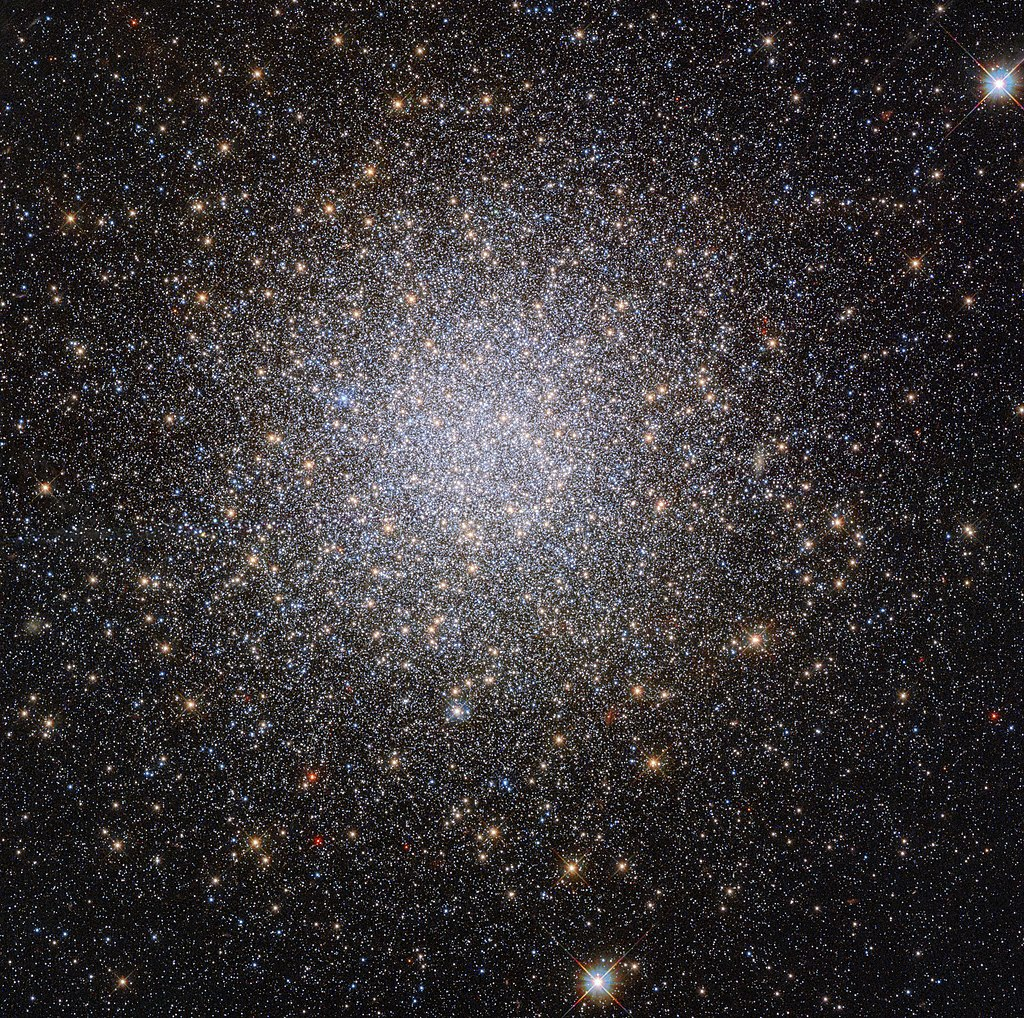
\includegraphics[width=3in]{Chapter-6/figs/NGC2419.jpg}
%\caption{\label{fig:NGC2419}An image of the globular cluster NGC 2419 taken by the Hubble Space Telescope \cite{NGC2419Hubble,Larsen2019}.}
%\end{figure}

\begin{figure}[t]
\centering
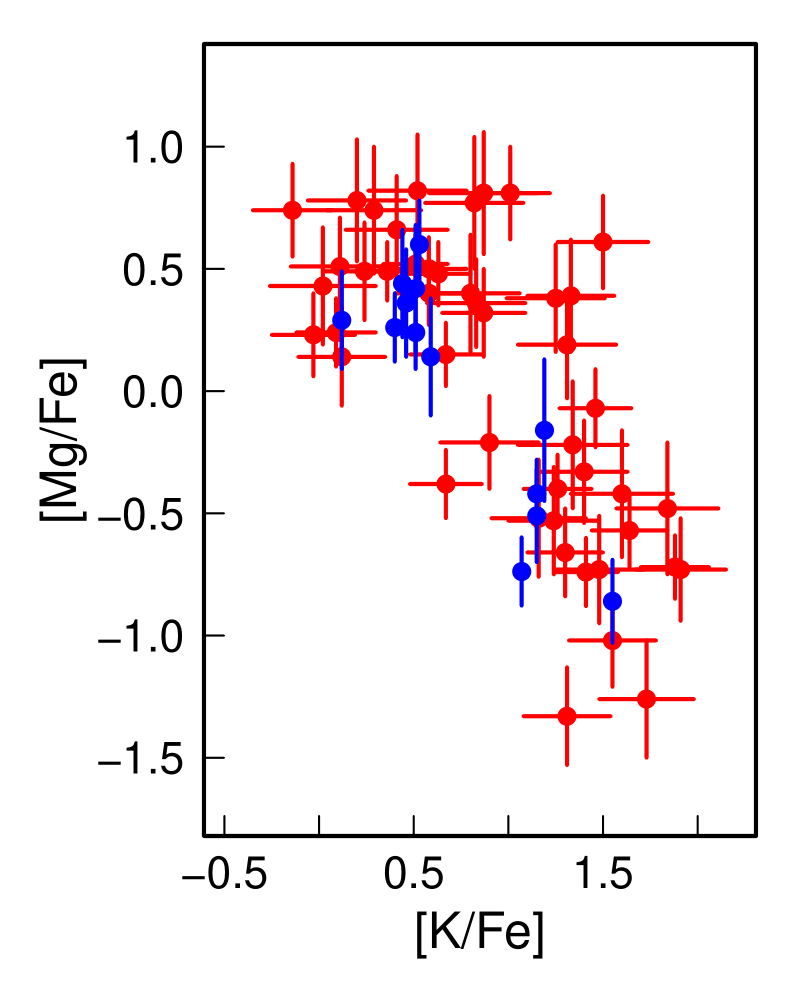
\includegraphics[width=2.5in]{Chapter-6/figs/MgK_Observation.png}
\caption{\label{fig:MgK}The observed Mg and K elemental abundances of red giants in NGC 2419 from Refs. \cite{Mucciarelli2012} (red) and \cite{Cohen2012} (blue). Figure adapted from \cite{Iliadis2016}.}
\end{figure}

% PARAGRAPH 2: Reaction network leading to K abundance (from 36Ar to 39K)

The hydrogen burning mechanism for the K enrichment in NGC 2419 has been shown to start from $^{36}$Ar, the most abundant argon isotope at such low metallicities \cite{Ventura2012}.

\begin{figure}[t]
\centering
\noindent
\begin{tikzpicture}[scale=1.75, every node/.style={transform shape}]

% (0,0) is at the bottom left corner of plot, where 36Ar is.
\filldraw[fill = light-gray] (0,0) rectangle (1,1); % 36Ar box
\draw (1+\BoxSpace,0) rectangle (2+\BoxSpace,1); % 37Ar box
\filldraw[fill = light-gray] (2+\BoxSpacetwo,0) rectangle (3+\BoxSpacetwo,1); % 38Ar box
\filldraw[fill = light-gray] (2+\BoxSpacetwo,-1-\BoxSpace) rectangle (3+\BoxSpacetwo,-\BoxSpace); % 37Cl box
\draw (0,1+\BoxSpace) rectangle (1,2+\BoxSpace); % 37K box
\draw (1+\BoxSpace,1+\BoxSpace) rectangle (2+\BoxSpace,2+\BoxSpace); % 38K box
\filldraw[fill = light-gray] (2+\BoxSpacetwo,1+\BoxSpace) rectangle (3+\BoxSpacetwo,2+\BoxSpace); % 39K box

\node at (0.5,0.5) {$^{36}\mathrm{Ar}$};
\node at (1+\BoxSpace+0.5,0.5) {$^{37}\mathrm{Ar}$};
\node at (2+\BoxSpacetwo+0.5,0.5) {$^{38}\mathrm{Ar}$};
\node at (0.5,1+\BoxSpace+0.5) {$^{37}\mathrm{K}$};
\node at (1+\BoxSpace+0.5,1+\BoxSpace+0.5) {$^{38}\mathrm{K}$};
\node at (2+\BoxSpacetwo+0.5,1+\BoxSpace+0.5) {$^{39}\mathrm{K}$};
\node at (2+\BoxSpacetwo+0.5,-\BoxSpace-0.5) {$^{37}\mathrm{Cl}$};

\draw[line width = \AW mm, -{Triangle[]}] (0.5,1-\AOS) -- (0.5,1+\BoxSpace+\AOS); % 36Ar(p,g)
\draw[line width = \AW mm, -{Triangle[]}] (1-\AOS,1+\BoxSpace+\AOS) -- (1+\BoxSpace+\AOS, 1-\AOS); % 37K(B+)
\draw[line width = \AW mm, -{Triangle[]}] (1+\BoxSpace+0.5,1-\AOS) -- (1+\BoxSpace+0.5,1+\BoxSpace+\AOS); % 37Ar(p,g)
\draw[line width = \AW mm, -{Triangle[]}] (2+\BoxSpace-\AOS,1+\BoxSpace+\AOS) -- (2+\BoxSpacetwo+\AOS,1-\AOS); %38K(B+)
\draw[line width = \AW mm, -{Triangle[]}] (2+\BoxSpacetwo+0.5,1-\AOS) -- (2+\BoxSpacetwo+0.5,1+\BoxSpace+\AOS); %38Ar(p,g)
\draw[line width = \AW mm, -{Triangle[]},dashed] (2+\BoxSpace-\AOS,\AOS) -- (2+\BoxSpacetwo+\AOS,-\BoxSpace-\AOS); %37Ar(EC)
\draw[line width = \AW mm, -{Triangle[]},dashed] (2+\BoxSpacetwo+0.5,-\BoxSpace-\AOS) -- (2+\BoxSpacetwo+0.5,\AOS); % 37Cl(p,g)

\end{tikzpicture}
%\vspace{0.75 cm}
\caption{\label{fig:KHBurning}The hydrogen burning mechanism driving the K enrichment in the globular cluster NGC 2419. The main nucleosynthesis chain is shown with solid arrows. The $^{37}\mathrm{Ar}(p, \gamma)^{38}\mathrm{K}$ reaction proceeds at a much higher rate than $^{37}\mathrm{Ar}(e^{-},\nu)^{37}\mathrm{Cl}$ electron capture, even at relatively low proton densities.}
\end{figure}

% PARAGRAPH 3: Ventura et al. (2012) polluter candidates

%Ventura \emph{et al.} \cite{Ventura2012} were the first to propose polluter star candidates for the Mg-K anticorrelation in NGC 2419. Hot-bottom burning in massive AGB stars and Super-AGB (SAGB) stars was considered, where temperatures can reach 150 MK, but many stellar model parameters would need adjusting.

% PARAGRAPH 4: Iliadis et al. (2016) monte carlo network calculations constraining temperature-density conditions and suggesting polluter candidates



% PARAGRAPH 5: Dermigny et al. (2017) reaction rate sensitivities suggesting 4 reactions are important



%%%%%%%%%%%%%%%%%%%%%%%%%%%%%%%%%%%%%%%%%%%%%%%%%%%%%%%%%%%%%%%%%%%%%%%%%%%%%%%%%%%%%%%%%%%%%
\section{$^{39}\mathrm{K}(p,\gamma)^{40}\mathrm{Ca}$}
% Longland et al. 2018

% PARAGRAPH 1: In particular, Dermigny et al. (2017) found that 39K(p,g)40Ca was important (with Longland et al. (2018)'s reaction rate, before the paper was published though)

\begin{figure}[t]
\centering
\noindent
\begin{tikzpicture}[scale=1.3, every node/.style={transform shape}]
\node at (0,0) {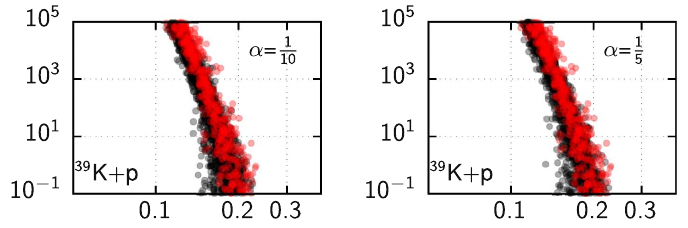
\includegraphics[scale=0.45]{Chapter-6/figs/39K_p_g_Sens1.png}};
\node at (0.04,-3.7) {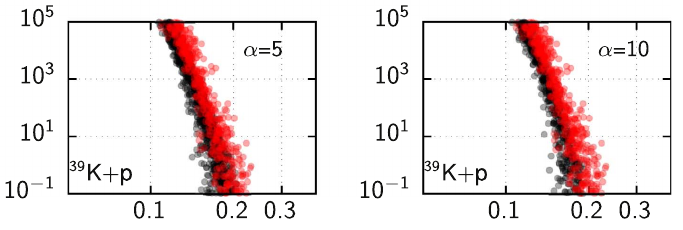
\includegraphics[scale=0.45]{Chapter-6/figs/39K_p_g_Sens2.png}};

\node at (0.3,-5.9) {Temperature (GK)};
\node[rotate=90] at (-5.7,-1.85) {Density ($\mathrm{g}/\mathrm{cm}^{3}$)};

\end{tikzpicture}

%\begin{subfigure}[t]{0.75\textwidth}
%	\centering
%	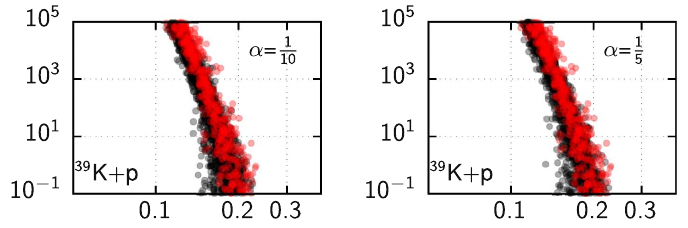
\includegraphics[width=1\linewidth]{Chapter-6/figs/39K_p_g_Sens1.png}
%\end{subfigure}
%\begin{subfigure}[t]{0.75\textwidth}
%	\centering
%   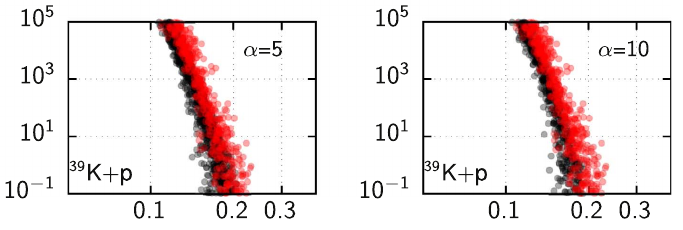
\includegraphics[width=1\linewidth]{Chapter-6/figs/39K_p_g_Sens2.png}
%\end{subfigure}

\caption{\label{fig:39K_p_g_Sens}Systematic effects of the $^{39}\mathrm{K}(p,\gamma)^{40}\mathrm{Ca}$ reaction rate influencing temperature-density conditions. The indicated variation factors ($\alpha = 1/10, 1/5, 5, 10$) are applied to the reaction rate in each panel, and the black dots show the resulting temperature-density conditions that provide an acceptable match with observed abundances. The red dots represent the case where no systematic effects ($\alpha=1$) have been added. Figure adapted from \cite{Dermigny2017}.}
\end{figure}

% PARAGRAPH 2: Longland et al. (2018) reaction rate calculation has many upper limits from unknown states, and the reaction rate uncertainty is very large in the Gamow window.

\begin{figure}[t]
\centering
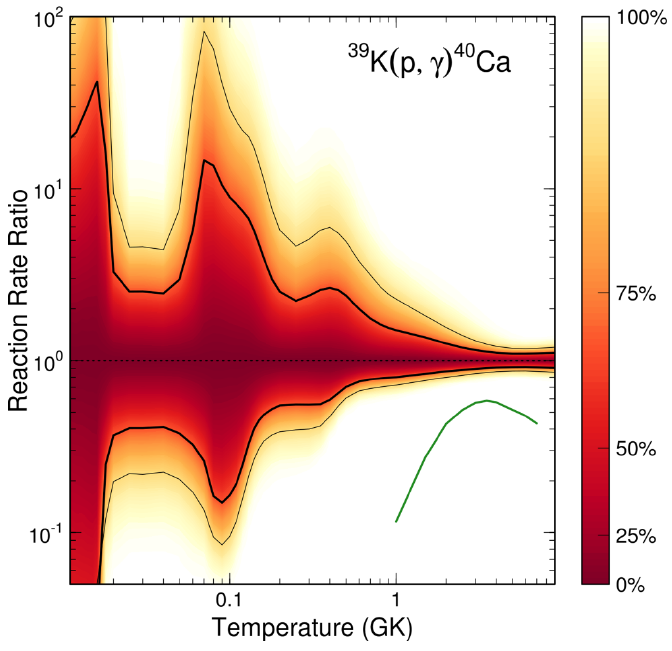
\includegraphics[width=4in]{Chapter-6/figs/39K_p_g_Longland2018.png}
\caption{\label{fig:39K_p_g_Longland}The recent $^{39}\mathrm{K}(p,\gamma)^{40}\mathrm{Ca}$ reaction rate probability density calculation of \cite{Longland2018} as a function of temperature. The median, recommended rate is shown as the dotted normalization line. The thick and thin black lines represent the $68\%$ ($1\sigma$) and $95\%$ ($2\sigma$) uncertainty bands, respectively. The color scale shows the continuous nature of the probability density, with darker red colors closer to the recommended rate. The green line represents the previous calculation of \cite{Cheng1981}.}
\end{figure}

% PARAGRAPH 3: No direct measurement for states below 8935 keV - Only 4 states measured below this through indirect measurements - 39K(3He,d)40Ca and 39K(d,n)40Ca, all between 1966 and 1971



% PARAGRAPH 4: This all motivates a 39K(p,g)40Ca reaction rate constraint. Using 39K(3He,d)40Ca lets us look at 39K+p states closer to the proton separation energy, which all contribute to the rate.

%%%%%%%%%%%%%%%%%%%%%%%%%%%%%%%%%%%%%%%%%%%%%%%%%%%%%%%%%%%%%%%%%%%%%%%%%%%%%%%%%%%%%%%%%%%%%
\section{Transfer Reaction Theory}

% Theory leading to C2S and proton partial-width calculations

%%%%%%%%%%%%%%%%%%%%%%%%%%%%%%%%%%%%%%%%%%%%%%%%%%%%%%%%%%%%%%%%%%%%%%%%%%%%%%%%%%%%%%%%%%%%%
\section{The $^{39}\mathrm{K}(^{3}\mathrm{He},d)^{40}\mathrm{Ca}$ Experiment}

% PARAGRAPH 1: Basically like the methods section in my 39K(3He,d)40Ca PRL paper, but go into much more detail about the tandem, enge, and detector setup.



% PARAGRAPH 2: Show an example spectrum with peaks labeled



% PARAGRAPH 3: Different spectra from the FP and Si detectors, including DE/E for particle discrimination.



%%% From PRL paper %%%
The $^{39}\mathrm{K}(^{3}\mathrm{He}, d)^{40}\mathrm{Ca}$ experiment was performed using the Enge Split-Pole Spectrograph at the Triangle Universities Nuclear Laboratory (TUNL). The 10 MV FN tandem Van de Graaff accelerator at TUNL accelerated a fully-ionized $^{3}$He beam to 21 MeV, where the energy was stabilized using a pair of high-resolution slits between two $90^{\circ}$ dipole magnets. The target was produced by evaporating approximately 75 $\mu\mathrm{g/cm}^{2}$ of natural potassium iodide onto an aluminum target frame with a 21 $\mu\mathrm{g/cm}^{2}$ natural carbon film backing. The $^{39}\mathrm{K}(^{3}\mathrm{He}, d)^{40}\mathrm{Ca}$ proton-transfer and $^{39}\mathrm{K}(^{3}\mathrm{He}, {}^{3}\mathrm{He})^{39}\mathrm{K}$ elastic scattering reactions were measured at lab angles between $5-20^{\circ}$ and $15-59^{\circ}$, respectively, using a focal-plane detector package \cite{Marshall2019} consisting of two position-sensitive avalanche counters, a $\Delta\mathrm{E}$ proportionality counter, and an E scintillator. The $\Delta\mathrm{E}/\mathrm{E}$ spectrum enables particle discrimination, allowing the position spectra to be gated on either $^{3}\mathrm{He}$ or $d$.

To minimize the effects of non-uniformity in the target, uncertainty in the target thickness, and target degradation after exposure to the beam, the $^{39}\mathrm{K}(^{3}\mathrm{He}, {}^{3}\mathrm{He})^{39}\mathrm{K}$ and $^{39}\mathrm{K}(^{3}\mathrm{He}, d)^{40}\mathrm{Ca}$ yields from the focal-plane detector were normalized to the simultaneous $^{39}\mathrm{K}(^{3}\mathrm{He}, {}^{3}\mathrm{He})^{39}\mathrm{K}$ yield of a Si detector telescope positioned at a constant $\theta_{\mathrm{lab}} = 45^{\circ}$ inside the target chamber. Normalizing to a global $^{3}\mathrm{He}$ optical model potential (OMP) for $^{39}\mathrm{K}$ then corrects the overall scale for the $^{39}\mathrm{K}(^{3}\mathrm{He}, d)^{40}\mathrm{Ca}$ differential cross-section.
%%%

%%%%%%%%%%%%%%%%%%%%%%%%%%%%%%%%%%%%%%%%%%%%%%%%%%%%%%%%%%%%%%%%%%%%%%%%%%%%%%%%%%%%%%%%%%%%%
\section{Bayesian Peak Fitting and Target Oxidation} \label{sec:peak_fitting}

% 1 paragraph overview first here...
The energy loss of light, charged particles through a medium is a statistical process. Particles with the same initial energy will traverse the same length in the medium with a distribution of final energies. This phenomenon is known as energy straggling and was theoretically described by Landau \cite{Landau}. Thin-film targets are ideal for high resolution spectral analysis because the energy loss distribution is approximately gaussian. Thick targets, however, alter the energy loss distribution in ways that present challenges to fitting peaks in a spectrum. Section \ref{subsec:peak_fitting_gaus} presents the Bayesian peak fitting procedure implemented in the analysis of the $^{39}\mathrm{K}(^{3}\mathrm{He}, d)^{40}\mathrm{Ca}$ experiment for the case of thin targets, and Section \ref{subsec:oxidation} presents a modified procedure for the case of thick targets, resulting from target oxidation which produces tails in the energy loss distribution.

\subsection{Bayesian Peak Fitting} \label{subsec:peak_fitting_gaus}

Transfer reaction analysis requires precise experimental cross section measurements for each relevant excited state of the residual nucleus. Each cross section is proportional to the yield of the transfer reaction populating the given excited state. An essential ingredient in the yield measurement, described in more detail in Section \ref{sec:cs_calc}, is the number of counts of ejectile particles measured by the focal-plane detector. Each count contributes to a peak along the focal-plane spectrum corresponding to the given excited state with a finite width. The peaks are distinguished by their excitation energies, which are determined through an energy calibration based on their relative centroid positions along the focal-plane, as is done in Section \ref{subsec:cal}. A typical transfer reaction spectrum will include many such peaks, as well as peaks from reactions in the target not necessarily of interest, known as contaminants. As mentioned in the introduction of this section, excited state peaks are typically gaussian-distributed, assuming a thin-film target is used. The spectrum will also include background counts, represented by a straight line. A precise determination of the number of counts in a given peak, in the simplest case, is therefore done by fitting a gaussian with a background line.

The target for the $^{39}\mathrm{K}(^{3}\mathrm{He}, d)^{40}\mathrm{Ca}$ experiment was natural potassium iodine on a natural carbon film backing. The most prominent contaminants were from $(^{3}\mathrm{He}, d)$ reactions on $^{12}$C, $^{13}$C, $^{14}$N, and $^{16}$O, producing excited states from the residual nuclei $^{13}$N, $^{14}$N, $^{15}$O, and $^{17}$F, respectively. The chosen magnetic field of the Enge Split-Pole Spectrograph was such that deuterons from $(^{3}\mathrm{He}, d)$ reactions with iodine were not at all present along the focal-plane, and deuterons from $^{41}\mathrm{K}(^{3}\mathrm{He}, d)$ were only minimally present. However, given the presence of the many other contaminants, and to distinguish doublets, triplets, and other mutliplets, it was deemed necessary to use a more sophisticated technique to fit the peaks from this experiment than a simple chi-squared minimization. Bayesian Monte Carlo sampling was a natural choice, considering its realistic uncertainty handling and flexibility when dealing with non-gaussian fits, presented in Section \ref{subsec:oxidation}. I used the \texttt{BayeSpec} \cite{BayeSpec} graphical user interface (GUI), along with custom Bayesian sampling routines described below, to acquire fits to the $^{39}\mathrm{K}(^{3}\mathrm{He}, d)^{40}\mathrm{Ca}$ data.

% BayeSpec GUI, MCMCGaus
Most peaks from transfer reactions on a thin-film target are gaussian-distributed,
\begin{equation}
    f(x;A,\mu,\sigma) = A \, \exp \Big( -\frac{(x-\mu)^{2}}{2\sigma^{2}} \Big),
\end{equation}
where $A$ is the peak intensity, $\mu$ is its mean, and $\sigma$ is its standard deviation.
%A chi-squared minimization would optimize these 3 parameters to fit the data. Alternatively, 
Bayesian sampling can be used to optimize these 3 parameters to match the focal-plane data if appropriate prior distributions are known. In this case, each prior distribution is approximately normal, $\mathcal{N}(\mu_{0},\sigma_{0}^{2})$, with its own mean $\mu_{0}$ and standard deviation $\sigma_{0}$. Posterior distributions can then be computed from these priors to achieve parameter values with statistically realistic uncertainties that match the data. These more realistic uncertainties make it possible to handle difficult fitting scenarios that would normally cause problems for chi-square minimizations, such as distinguishing peaks in a multiplet with appropriate uncertainties.

Prior means $\mu_{0}$ for $A$ and $\mu$ are particularly simple to obtain if the peak apex is visible. Even if it is not visible, as in the case of a multiplet, a guess can be made for each peak apex location, $(x,y)$, based on the curvature of their sum, where $x$ is the mean guess and $y$ is the intensity guess. Each guess is established by selecting a point using the \texttt{BayeSpec} GUI. The prior standard deviations $\sigma_{0}$ for $A$ and $\mu$ are given constant values conservative enough for sampling to be successful in even the most uncertain cases. These can be adjusted by the user, but are typically left as their defaults.

The prior mean $\mu_{0}$ and standard deviation $\sigma_{0}$ for $\sigma$ are ideally given constant values for a given reaction representative of most peaks from that reaction in focal-plane spectra. This is because energy loss is nearly equivalent for peaks with similar excitation energies from the same reaction, but it is not equivalent for peaks from different reactions. Therefore, peaks from each reaction should ideally have a shared $\sigma$ prior and a shared $\sigma$ posterior in a single fit if multiple peaks are fit simultaneously. In practice, a single $\sigma$ prior can be used for different reactions if it is conservative enough for sampling to be successful, but the $\sigma$ posteriors should remain different for different reactions. 

A background line must also be included in the model, where its intensity $y_{\mathrm{bg}}$ and slope $m_{\mathrm{bg}}$ have their own $\mathcal{N}(\mu_{0}, \sigma_{0}^{2})$ priors. Put together, the prior distributions for gaussian peaks on a background line in a typical focal-plane spectrum are
\begin{align}
    A_{i} &\sim \mathcal{N}(y_{i}, 10.0^{2}) \nonumber \\
    \mu_{i} &\sim \mathcal{N}(x_{i}, 1.0^{2}) \nonumber \\
    \sigma &\sim \mathcal{N}(5.0, 1.0^{2}) \nonumber \\
    y_{\mathrm{bg}} &\sim \mathcal{N}(\mathrm{max}(1, \mathrm{min}(d)), 0.1^{2}) \nonumber \\
    m_{\mathrm{bg}} &\sim \mathcal{N}(0, 0.01), \label{eqn:gaus_priors}
\end{align}
where $\sigma$ is a constant prior for all reactions, but it can easily be adjusted by the user for different reactions if needed, and $d$ refers to the focal-plane data in the specified fit range. The prior for $m_{\mathrm{bg}}$ can also be adjusted if the background line is clearly not horizontal. The model function to be fit is
\begin{equation}
    f(x;A,\mu,\sigma,y_{\mathrm{bg}},m_{\mathrm{bg}}) = \sum_{i}^{N} A_{i} \, \exp \Big( -\frac{(x-\mu_{i})^{2}}{2\sigma_{\hspace{-0.08cm} j}^{2}} \Big) + \Big(y_{\mathrm{bg}} + m_{\mathrm{bg}} (x - \mathrm{min}(x))\Big), \label{eqn:nGausBkg}
\end{equation}
where $N$ is the total number of gaussian peaks to be fit and $\sigma_{\hspace{-0.08cm} j}$ refers to the shared standard deviation for peaks from reaction $j$.

The posterior computation in the custom Bayesian sampling routine uses the \texttt{quap} function in \texttt{R}, part of the Bayesian \texttt{rethinking} package from Richard McElreath \cite{McElreath2020}. This function finds a quadratic approximation to each full posterior distribution at its mode. It is less sophisticated than Markov Chain Monte Carlo, but its relative simplicity makes it a more efficient option to use with a GUI. The model composed of Eqns. \ref{eqn:gaus_priors} and \ref{eqn:nGausBkg} is provided to \texttt{quap}, which returns the posterior quadratic approximations with built-in uncertainties. Samples from these posteriors are then used to compute the area of each gaussian, given by $\sqrt{2\pi} \, \sigma_{\hspace{-0.08cm} j} A_{i}$, along with their uncertainties. A small number of posterior samples are also used to graphically display the gaussian fits, with different colors representing different reactions.

Figure \ref{fig:Gaus_Bayesian} shows an example of this Bayesian fitting procedure for a $^{39}\mathrm{K}(^{3}\mathrm{He},d)^{40}\mathrm{Ca}$ focal-plane spectrum at $\theta_{\mathrm{lab}} = 5^{\circ}$. Excited states of $^{40}\mathrm{Ca}$ are shown in red and $^{14}\mathrm{N}$ excited state contaminants are shown in orange. In blue is the sum of the gaussians and the background line, given by Eqn. \ref{eqn:nGausBkg}. Each gaussian, as well as the blue curve, consists of 50 individual curves that were sampled from the posteriors to represent the uncertainties. The reason it is useful to combine these 4 peaks into one fit in this example is to better resolve the 5903 keV $^{40}$Ca state in red from the 4915 keV $^{14}$N state in orange in the double gaussian on the right side of the spectrum. The addition of the 6025 keV $^{40}$Ca peak in red and the 5106 keV $^{14}$N peak in orange on the left constrains the $\sigma$ posteriors for the double gaussian. While this may seem like a minor correction, and it is minor in the present example, it is crucial in situations where the double gaussian or multiplet is otherwise impossible to resolve.

\begin{figure*}[t]
\centering
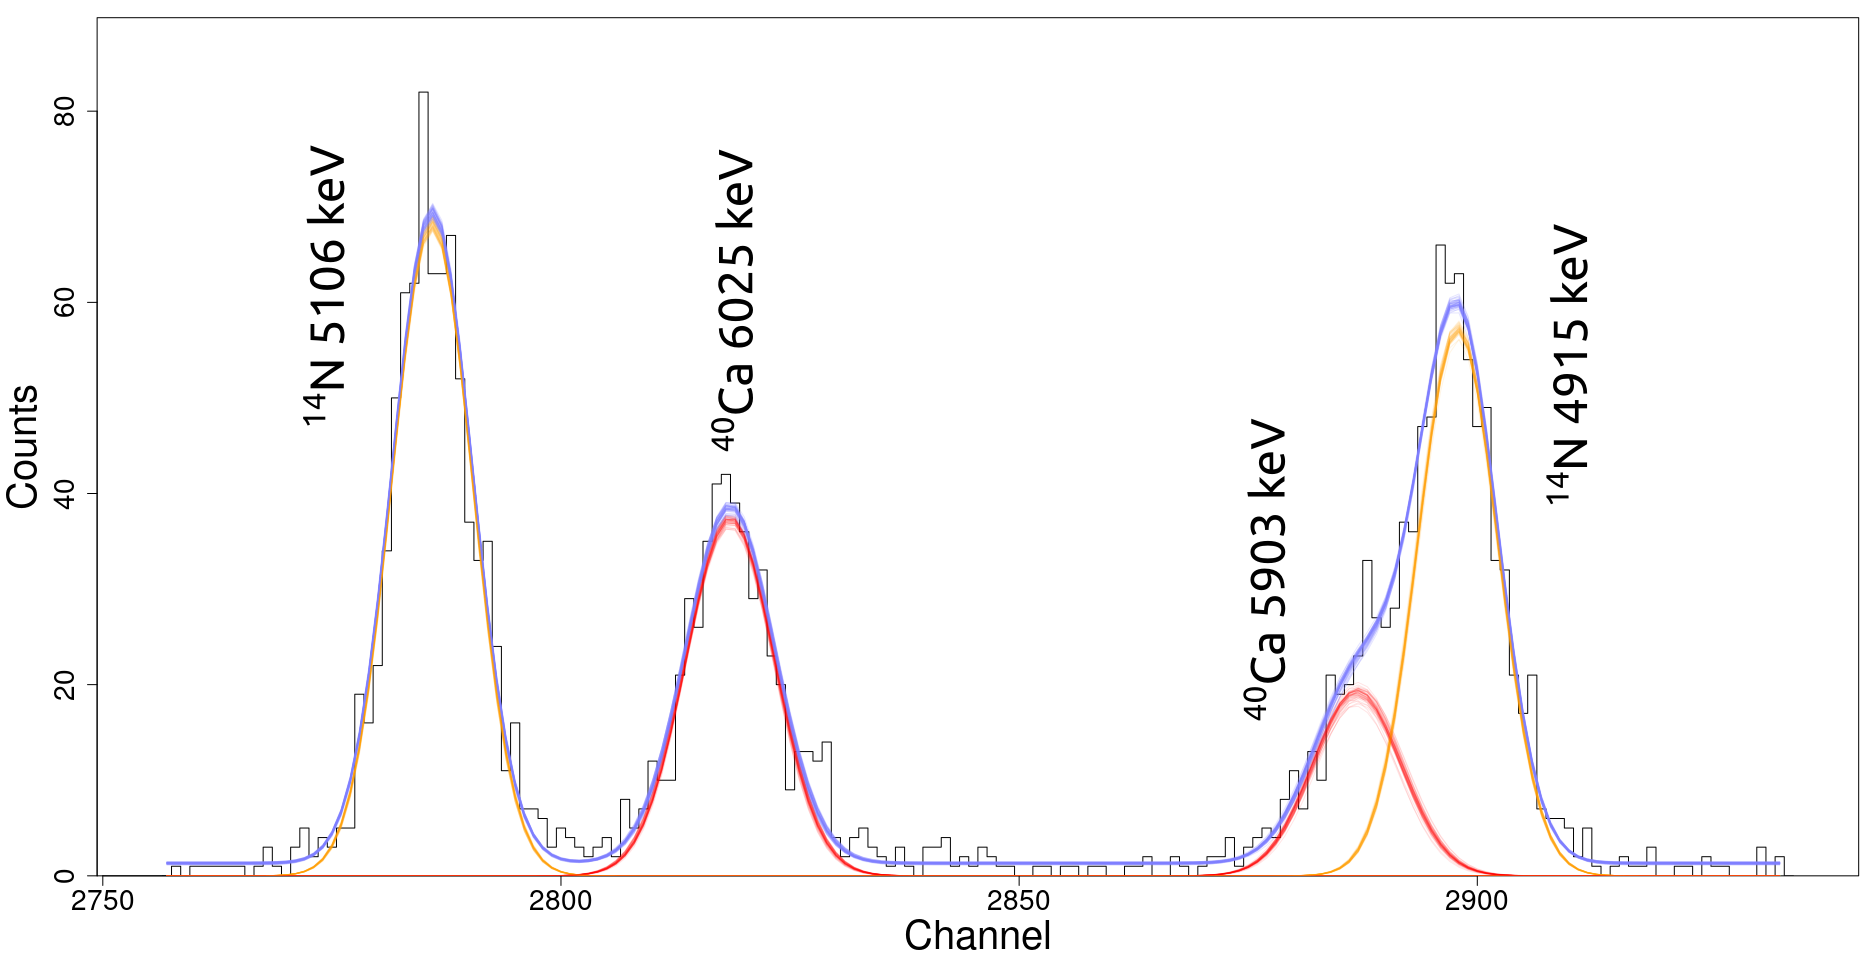
\includegraphics[width=6.5in]{Chapter-6/figs/Gaus_Bayesian.png}
\caption{\label{fig:Gaus_Bayesian}A Bayesian multi-gaussian fit with \texttt{BayeSpec} for the $^{40}$Ca excited states (in red) 6025 keV and 5903 keV from $^{39}\mathrm{K}(^{3}\mathrm{He},d)^{40}\mathrm{Ca}$ and the $^{14}$N excited states (in orange) 5106 keV and 4915 keV from $^{13}\mathrm{C}(^{3}\mathrm{He},d)^{14}\mathrm{N}$ at $\theta_{\mathrm{lab}} = 5^{\circ}$. In red and orange are 50 random samples of the gaussian distributions from the $\sigma$, $\mu$, and $A$ posteriors for each peak. The $^{40}$Ca peaks share an identical $\sigma$ posterior, while the $^{14}$N peaks share their own as well. In blue are the sums of the peaks plus the background line for each of those 50 samples.}
\end{figure*}

%%*****************************************************************************************%%
\subsection{Fitting Peaks with Target Oxidation} \label{subsec:oxidation}

Potassium iodine is hygroscopic, meaning it easily absorbs moisture from the environment. When exposed to atmospheric pressure, the salt slowly oxidizes, forming potassium carbonate and molecular iodine. This oxidation increases the thickness of thin-film targets. The probability of particles traversing the target with large final energies is decreased, introducing a high energy tail in the ejected particle spectrum. The Landau distribution describes this energy loss, but it is computationally challenging to implement. An approximation that has been found to fit oxidized-target spectra well is the exponentially-modified gaussian (EMG) distribution \cite{Babu2016}. The power of the EMG approximation is that its area calculation is the exact same as that of a gaussian distribution, $\sqrt{2\pi} \, \sigma A$, where $\sigma$ and $A$ are parameters of both gaussians and EMGs, but they have slightly different definitions as it will become clear below. This makes it very simple to determine the number of counts for EMG distributions, unlike Landau distributions, where the full area integral must be calculated.

% What to do when the target is oxidized and therefore the peaks have high energy tails. This is called energy straggling and is physically described by the Landau distribution. An approximation to this is an exponentially-modified gaussian 
% Cite: [Measurement of Energy Loss Straggling of Relativistic Electrons in Thin Aluminum Foils, S. Ramesh Babu and N.M. Badiger, ACTA Physica Polonica A. Vol. 129 (2016) DOI: 10.12693/AphysPolA.129.1118  | Page 1119 Section 2.2: Straggling theories of thin absorbers]

The probability density function (PDF) of an EMG distribution $f$ is a convolution of exponential $g$ and gaussian $h$ PDFs,
\begin{align}
    f(x;\sigma,\lambda,\mu,A) = (g*h)(x) &= \int_{-\infty}^{\infty}g(x')h(x-x') \, dx' \nonumber \\
             &= \int_{0}^{\infty}\lambda \exp\big(-\lambda x'\big) \, A\exp\Big(-\frac{1}{2}\Big(\frac{x-x'-\mu}{\sigma}\Big)^{2}\Big) \, dx' \nonumber \\
             &= A \, \sigma\lambda\sqrt{\frac{\pi}{2}}\exp\Big(\frac{1}{2}(\sigma\lambda)^{2} - (x-\mu)\lambda\Big) \, \mathrm{erfc}\Big(\frac{1}{\sqrt{2}}\Big(\sigma\lambda - \frac{x-\mu}{\sigma}\Big)\Big),
\end{align}
where $\lambda$ is the exponential-component rate, $\mu$, $\sigma$, and $A$ are the gaussian-component mean, standard deviation, and peak intensity, respectively, and $\mathrm{erfc}$ is the complimentary error function, defined as $\mathrm{erfc} \, z = 1 - \mathrm{erf} \, z$ for the complex variable $z$, where $\mathrm{erf}$ is the error function,
\begin{equation}
    \mathrm{erf} \, z = \frac{2}{\sqrt{\pi}}\int_{0}^{z}\exp\big(-t^2\big) \, d t.
\end{equation}
The standard EMG distribution, as a function of $x$, has a high--$x$ tail. Since the focal-plane position spectrum channel number is inversely related to energy, the EMG must be modified to have a low--$x$ tail. This is done by simply replacing $x-\mu$ with $\mu-x$ to reflect the standard EMG distribution about its gaussian-component mean, $\mu$. The following discussion of EMG distributions assumes this reflection has been performed.

Previously it was shown for non-oxidized targets that the Bayesian fitting procedure for a gaussian peak requires gaussian mean $\mu$ and peak intensity $A$ priors. The means of these priors are provided by the user when selecting an estimate at the peak apex with the \texttt{BayeSpec} GUI. However, this presents a problem when extending the procedure to EMG fits. An EMG is defined by the $\mu$ and $A$ parameters of its gaussian component, not the mean and peak intensity of the EMG itself. To obtain reasonable priors for the $\mu$ and $A$ parameters, they must be derived from the attributes of the EMG peak apex, where the user selects. This apex defines the mode $x_{m}$ and peak intensity $y_{m}$ of the EMG, which can both be calculated by determining the coordinates where the derivative of the PDF is equal to zero. These are
%The simplest attributes of an EMG from the perspective of the user are the mode $x_{m}$ and peak intensity $y_{m}$, which can also be calculated by determining the coordinates where the derivative of the PDF is equal to zero. These are
\begin{align}
    x_{m} &= \mu - \sigma^{2}\lambda + \sqrt{2} \, \sigma \, z, \nonumber \\
    y_{m} &= A \, \exp \Big( -\frac{1}{2} \Big( \frac{\mu - x_{m}}{\sigma} \Big)^{2} \Big), \label{eqn:mode_peak_intensity}
\end{align}
where $z$ is defined such that
\begin{equation}
    \exp(z^{2}) \, \mathrm{erfc}(z) = \sqrt{\frac{2}{\pi}} \, \frac{1}{\sigma\lambda},
\end{equation}
which can be solved numerically. With $x_{m}$ and $y_{m}$ provided by the user, $\mu$ and $A$ become
\begin{align}
    \mu(\sigma, \lambda) &= x_{m} + \sigma^{2} \lambda - \sqrt{2} \sigma z, \label{eqn:mu_before} \\
    A(\sigma, \lambda) &= y_{m} \exp \Big( \frac{1}{2} \Big( \frac{\mu-x_{m}}{\sigma} \Big)^{2} \Big). \label{eqn:A_before}
\end{align}
\begin{figure*}[t]
    \centering
    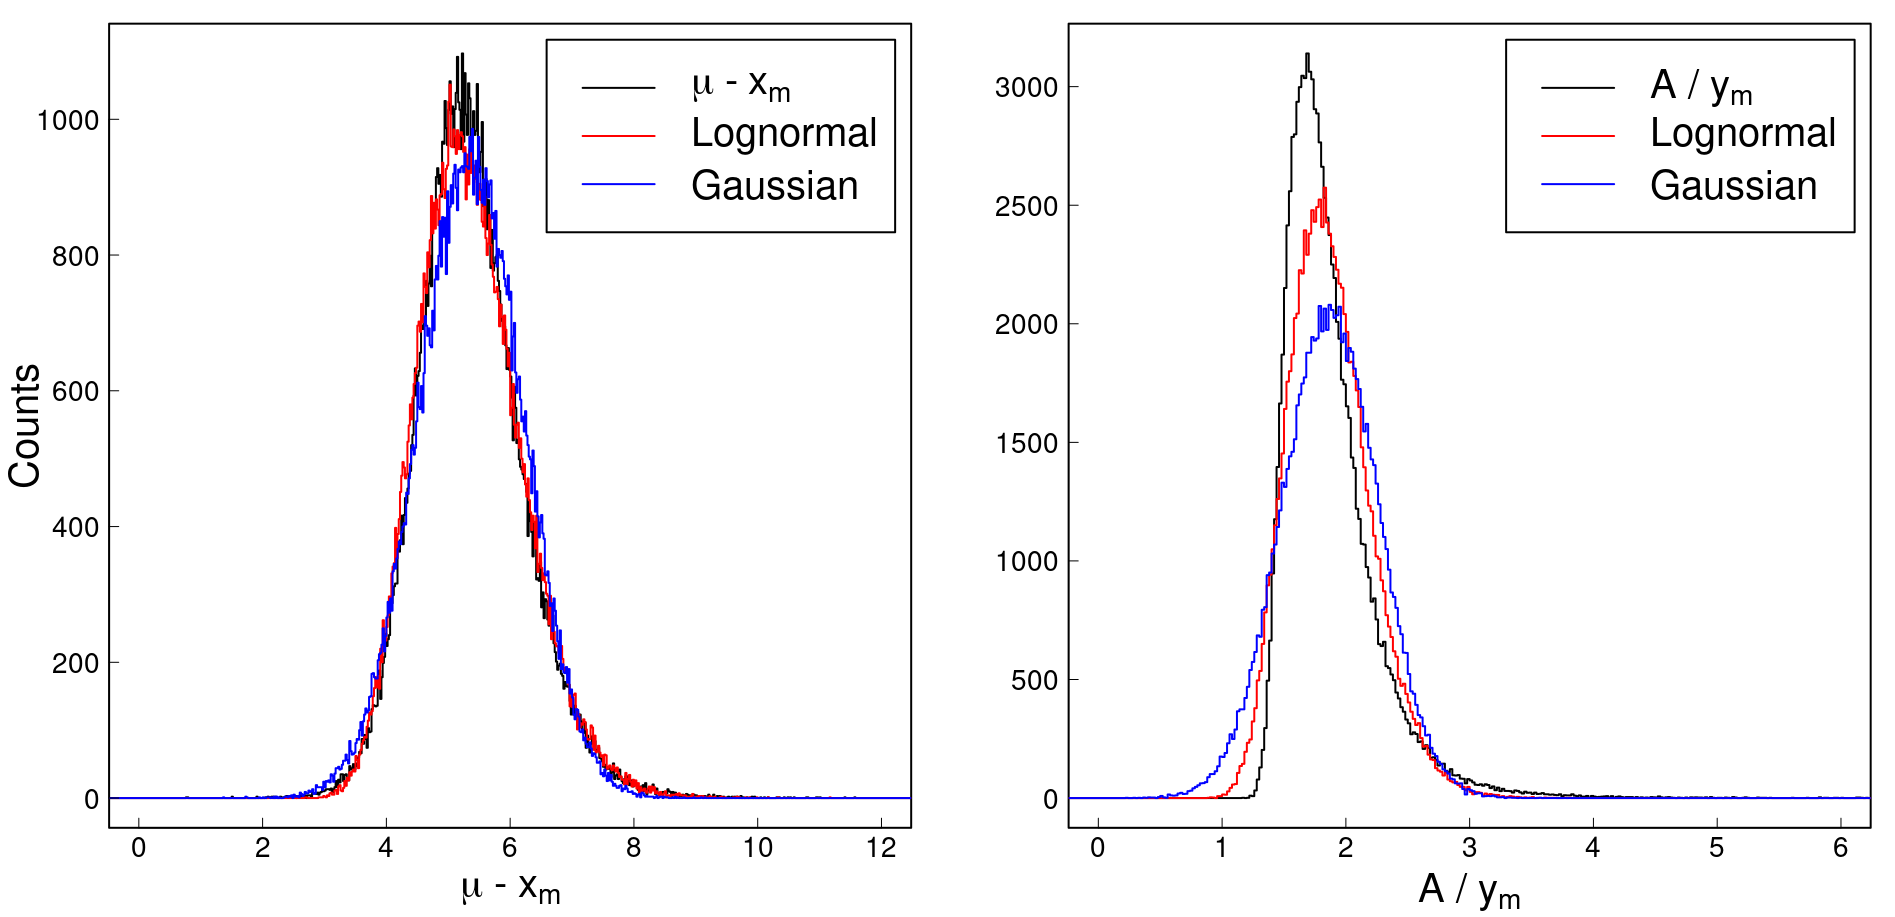
\includegraphics[width=6.5in]{Chapter-6/figs/mu_and_A.png}
    \caption{\label{fig:mu_and_A}The constructed priors for $\mu - x_{m}$ (left) and $A/y_{m}$ (right) from 10,000 samples of the $\sigma$ and $\lambda$ priors of Eqns. \ref{eqn:sig_prior} and \ref{eqn:lambda_prior}. The gaussian (blue) approximations were derived from the mean and standard deviation of the samples. The lognormal (red) approximations were derived from the mean and standard deviation of the natural logarithm of those samples.}
\end{figure*}
The priors would be fully determined if $\sigma$ and $\lambda$, the parameters related to the EMG width and skewness, can be constrained. Fortunately, for a given transfer reaction observed in a focal-plane spectrum, there is little variation between these properties, much like the gaussian $\sigma$ parameter of Section \ref{subsec:peak_fitting_gaus}. From a sample of EMG fits for $^{39}\mathrm{K}(^{3}\mathrm{He},d)^{40}\mathrm{Ca}$ peaks, reasonable priors for $\sigma$ and $\lambda$ were determined to be
\begin{align} 
    \sigma &\sim \mathcal{N}(5.0, \, 1.0^{2}), \label{eqn:sig_prior} \\
    \lambda &\sim \mathcal{N}(0.09, \, 0.02^{2}), \label{eqn:lambda_prior}
\end{align} 
where these are also usually sufficient for other reactions. Priors for Eqns. \ref{eqn:mu_before} and \ref{eqn:A_before} can then be constructed by sampling from Eqns. \ref{eqn:sig_prior} and \ref{eqn:lambda_prior}. The resulting prior distributions for $\mu - x_{m}$ and $A / y_{m}$ are shown in Figure \ref{fig:mu_and_A} in black after taking 10,000 samples from Eqns. \ref{eqn:sig_prior} and \ref{eqn:lambda_prior}. The gaussian approximations (blue) were constructed from the mean and standard deviation of the $\mu - x_{m}$ and $A/y_{m}$ samples, while the lognormal approximations (red) were similarly constructed from the mean and standard deviation of the natural logarithm of those samples. Note that the priors are not gaussian. In fact, the prior for $A / y_{m}$ is neither gaussian nor lognormal. However, a lognormal approximation suffices for both in practice and is preferable to the actual distributions, which are either non-analytical or at least exceedingly complicated. The Bayesian quadratic approximation function, \texttt{quap}, used with \texttt{BayeSpec} requires named prior distributions, forbidding the use of non-analytical distributions. The lognormal approximations also correctly prevent negative sample values and are therefore taken as the priors for $\mu$ and $A$.

\begin{figure*}[t]
\centering
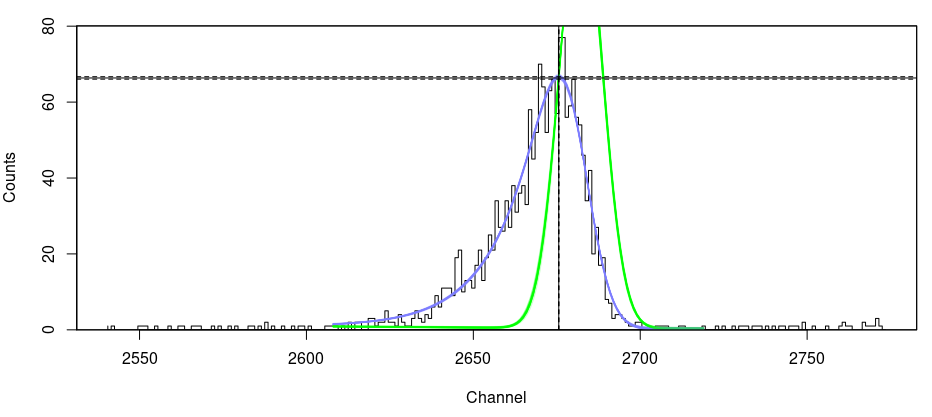
\includegraphics[width=6.5in]{Chapter-6/figs/ExpModGauss_Mode_and_Intensity.png}
\caption{\label{fig:EMG_Mode}A Bayesian exponentially-modified gaussian fit with \texttt{BayeSpec} for the 6285 keV $^{40}\mathrm{Ca}$ state from $^{39}\mathrm{K}(^{3}\mathrm{He},d)^{40}\mathrm{Ca}$ at $\theta_{\mathrm{lab}} = 5^{\circ}$ with an oxidized potassium iodine target. In blue are 50 random samples of the exponentially-modified gaussian distribution from the $\sigma$, $\lambda$, $\mu$, and $A$ posteriors, plus the background line. In green are the gaussian components of the exponentially-modified gaussian samples. The new mode and peak intensity are represented by the black lines, where the solid line represents their mean and the dashed lines represent their standard deviation.}
%The mode and peak intensity means of the 10,000 samples are shown by solid black lines, while their standard deviations are represented by dashed lines.
\end{figure*}

As in Section \ref{subsec:peak_fitting_gaus}, once the priors have been determined, the quadratic approximations to the posteriors are computed with \texttt{quap}, and the fit is constructed from samples of the EMG distribution with those posteriors. An example of this Bayesian EMG fitting method is shown in Figure \ref{fig:EMG_Mode}, where the 6285 keV $^{40}$Ca state from $^{39}\mathrm{K}(^{3}\mathrm{He},d)^{40}\mathrm{Ca}$ at $\theta_{\mathrm{lab}} = 5^{\circ}$ is fit with an EMG distribution because the potassium iodine target for this run had undergone oxidation. %The $\mu$ and $A$ priors of Eqns. \ref{eqn:mu_before} and \ref{eqn:A_before} were obtained by taking 10,000 samples from the $\sigma$ and $\lambda$ priors of Eqns. \ref{eqn:sig_prior} and \ref{eqn:lambda_prior} and approximating this as a lognormal distribution. 
The closely-packed blue lines are 50 representative samples of the EMG posteriors, plus that of the background line, while the green lines are the corresponding gaussian components of those EMG samples with mean $\mu$, standard deviation $\sigma$, and peak intensity $A$. The new mode and peak intensity from Eqn \ref{eqn:mode_peak_intensity}, obtained by sampling from the posteriors, are shown by the black lines, where the solid line represents its mean and the dashed lines represent its standard deviation. Note that the ($x_{m}$, $y_{m}$) coordinate lies along its gaussian component, a ubiquitous property of EMG distributions. The number of counts in the EMG distribution is simply equivalent to the area of its gaussian component, $\sqrt{2\pi} \, \sigma A$, constructed by sampling from the $\sigma$ and $A$ posteriors.

Figure \ref{fig:EMG_Multiplet} shows how powerful this method can be for high resolution spectral analysis with an oxidized target. The same focal-plane spectrum as Figure \ref{fig:EMG_Mode} is shown here, but it is focused on a region with multiple peaks. The blue summed fit consists of 5 EMG distributions, shown individually by the red and orange lines, and a small, virtually horizontal background line. As before, each distribution shows 50 lines drawn from samples of the EMG posteriors. From a simple energy calibration, the red peaks were found to be $^{40}$Ca excited states with excitation energies 7694 keV, 7658 keV, 7623 keV, and 7532 keV, from left to right, and the orange peak corresponds to the $^{14}$N 6446 keV excited state. Because we expect energy loss to be nearly equivalent for peaks with similar energies from the same reaction, the $\sigma$ and $\lambda$ width and skewness parameter posteriors are fixed between the $^{40}$Ca peaks, while the $^{14}$N peak has its own $\sigma$ and $\lambda$ posteriors. The custom Bayesian sampling routines for both gaussian and EMG fits can be used for a simultaneous fit of any number of peaks from up to 3 different reactions at present, and this could easily be extended to any number of reactions when the need arises.

\begin{figure*}[t]
\centering
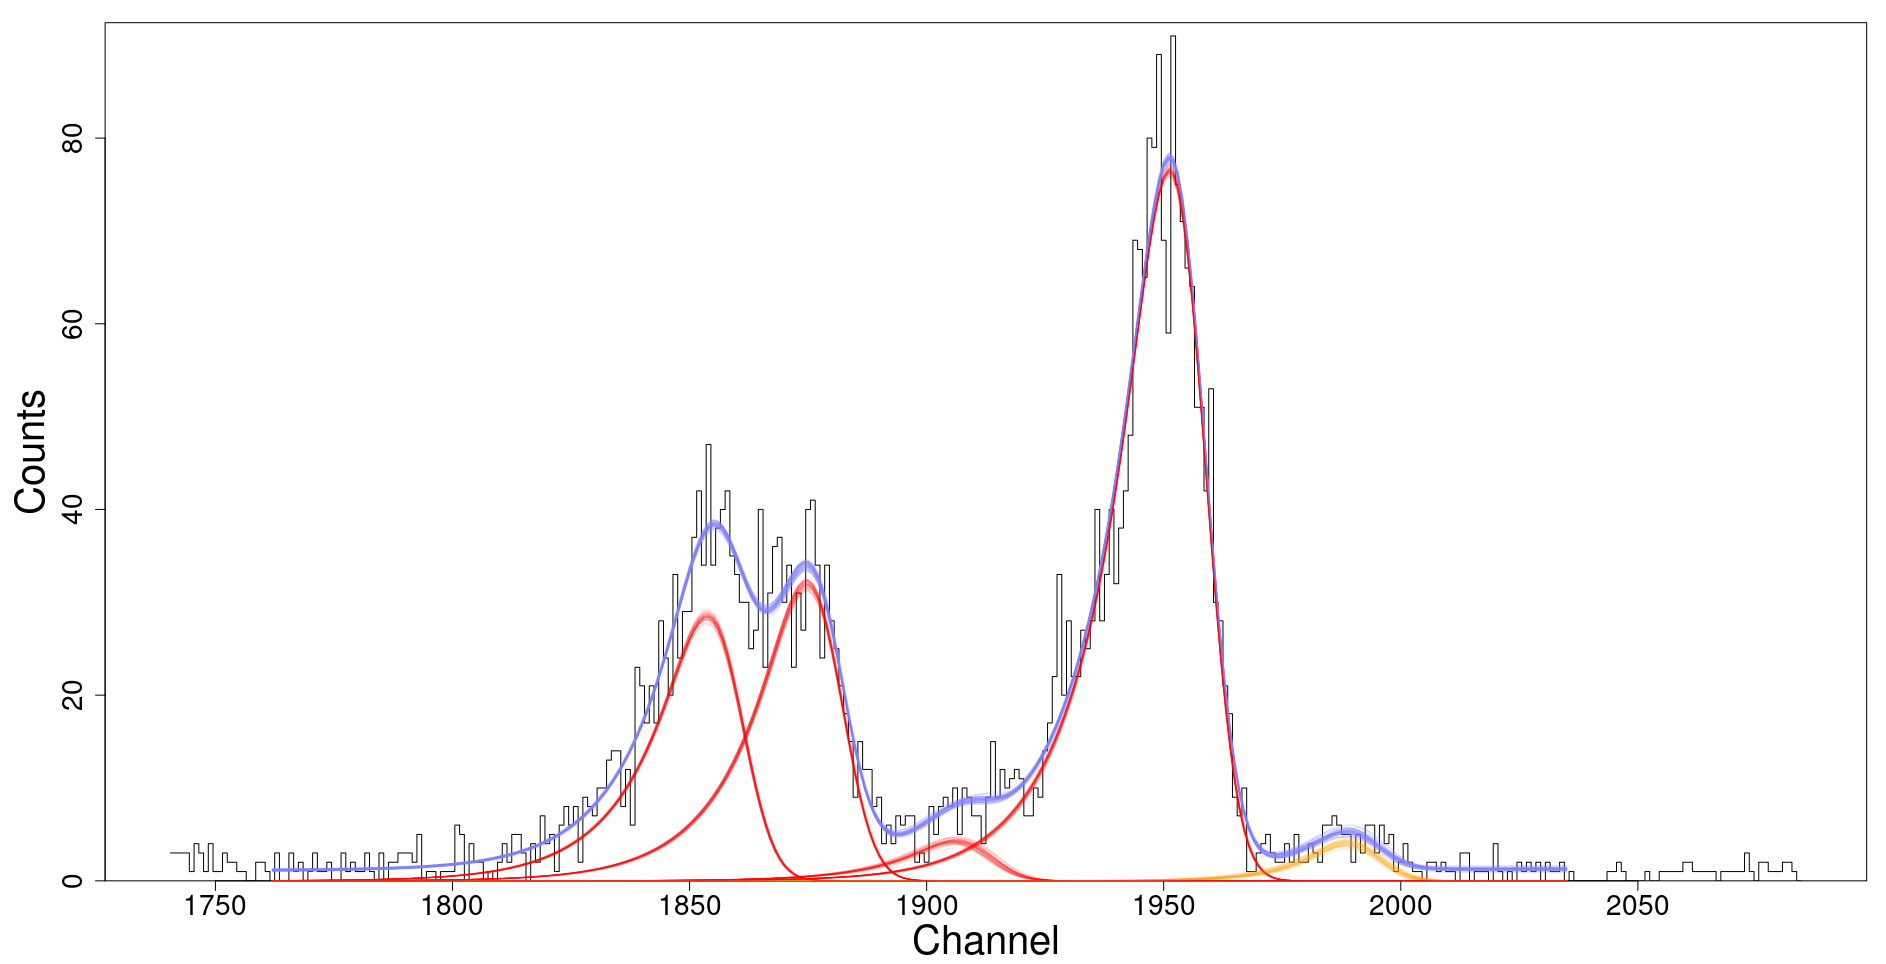
\includegraphics[width=6.5in]{Chapter-6/figs/EMG_Multiplet.png}
\caption{\label{fig:EMG_Multiplet}A Bayesian exponentially-modified gaussian fit with \texttt{BayeSpec} for the $^{40}$Ca excited states (left to right, in red) 7694 keV, 7658 keV, 7623 keV, and 7532 keV from $^{39}\mathrm{K}(^{3}\mathrm{He},d)^{40}\mathrm{Ca}$ and the $^{14}$N excited state (in orange) 6446 keV from $^{13}\mathrm{C}(^{3}\mathrm{He},d)^{14}\mathrm{N}$ at $\theta_{\mathrm{lab}} = 5^{\circ}$ with an oxidized potassium iodine target. In red and orange are 50 random samples of the exponentially-modified gaussian distributions from the $\sigma$, $\lambda$, $\mu$, and $A$ posteriors for each peak. The $^{40}$Ca peaks share identical $\sigma$ and $\lambda$ posteriors, whereas the $^{14}$N peak has its own. In blue are the sums of the peaks plus the background line for each of those 50 samples.}
\end{figure*}

%Since $x_{m}$ and $y_{m}$ are constant, they can be added and multiplied, respectively, to the resulting normal distributions from the following properties. Consider a normally distributed random variable $X$ with mean $a$ and variance $b^2$. Then the properties
%\begin{align}
%    X + c &\sim \mathcal{N}(a+c,b^{2}), \label{norm_prop1} \\
%    cX &\sim \mathcal{N}(ca,c^{2}b^{2}), \label{norm_prop2}
%\end{align}
%follow from the PDF of the normal distribution for a constant $c$. 

%Taking 10,000 samples from Eqns. \ref{sig_prior} and \ref{lambda_prior}, and using Eqns. \ref{norm_prop1} and \ref{norm_prop2}, Eqns. \ref{mu_before} and \ref{A_before} become
%\begin{align}
%    \mu &\sim \mathcal{N}(x_{m} + 5.37, \, 0.862^{2}) \\
%    A &\sim \mathcal{N}(1.87 y_{m}, \, 0.362^{2} y^{2}_{m}).
%\end{align}

%\begin{equation}
%    z = \mathrm{erfcxinv}\Bigg(\sqrt{\frac{2}{\pi}} \, \frac{1}{\sigma\lambda}\Bigg).
%\end{equation}
%The function $\mathrm{erfcxinv}$ is the inverse of the scaled complementary error function $\mathrm{erfcx}$, defined as
%\begin{equation}
%    \mathrm{erfcx}(z) = \exp(z^{2}) \, \mathrm{erfc}(z).
%\end{equation}
%In other words, $z$ is obtained by sol

%%*****************************************************************************************%%

%%%%%%%%%%%%%%%%%%%%%%%%%%%%%%%%%%%%%%%%%%%%%%%%%%%%%%%%%%%%%%%%%%%%%%%%%%%%%%%%%%%%%%%%%%%%%
\section{Cross Section Calculations and Si Detector Normalization} \label{sec:cs_calc}

% Short introduction here...

\subsection{Cross Sections}

\subsection{Si Detector Normalization}


%%%%%%%%%%%%%%%%%%%%%%%%%%%%%%%%%%%%%%%%%%%%%%%%%%%%%%%%%%%%%%%%%%%%%%%%%%%%%%%%%%%%%%%%%%%%%
\section{$^{39}\mathrm{K}(^{3}\mathrm{He},d)^{40}\mathrm{Ca}$ Analysis}

\subsection{Energy Calibrations} \label{subsec:cal}



\subsection{Cross Sections}

\begin{figure*}[t]
\centering
%\begin{tikzpicture}
%%\hspace{0.3cm}
%\node at (-4,0) {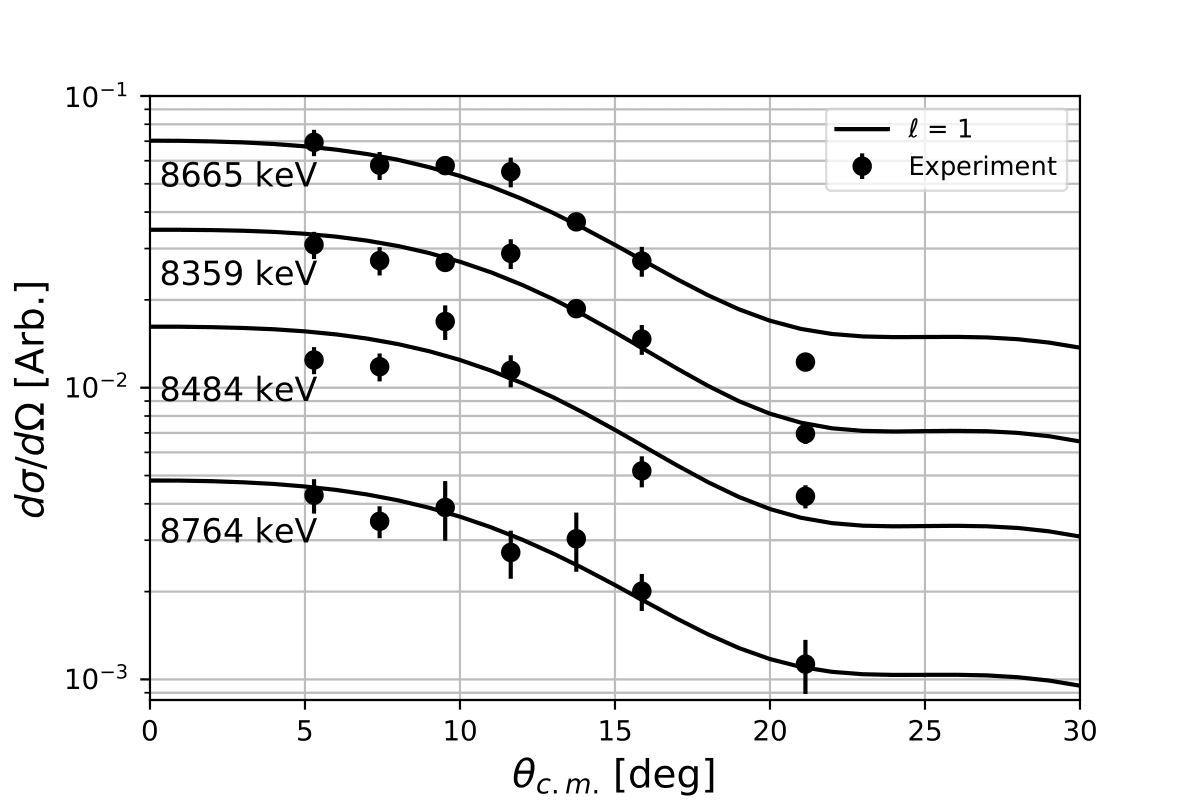
\includegraphics[width=8.6cm]{Chapter-4/figs/unbound_l1.png}};
%\node at (4,0) {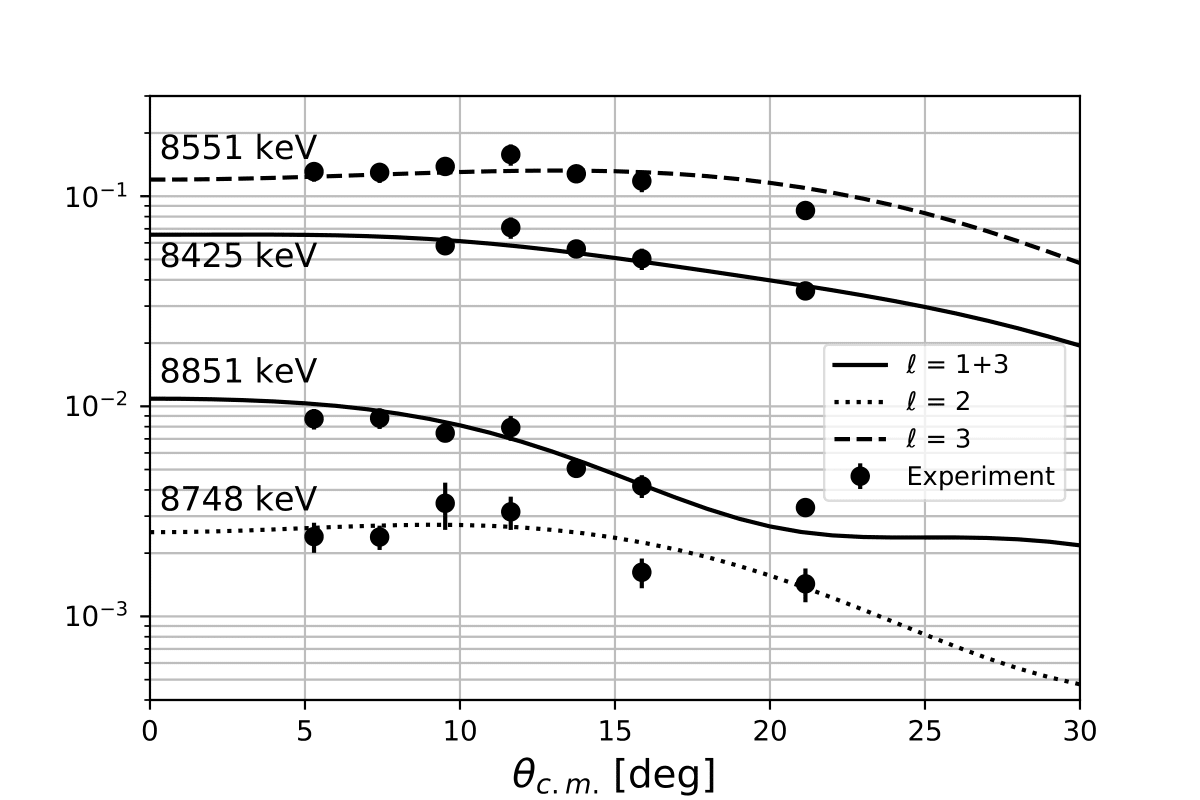
\includegraphics[width=8.6cm]{Chapter-4/figs/unbound_others.png}};
%\end{tikzpicture}
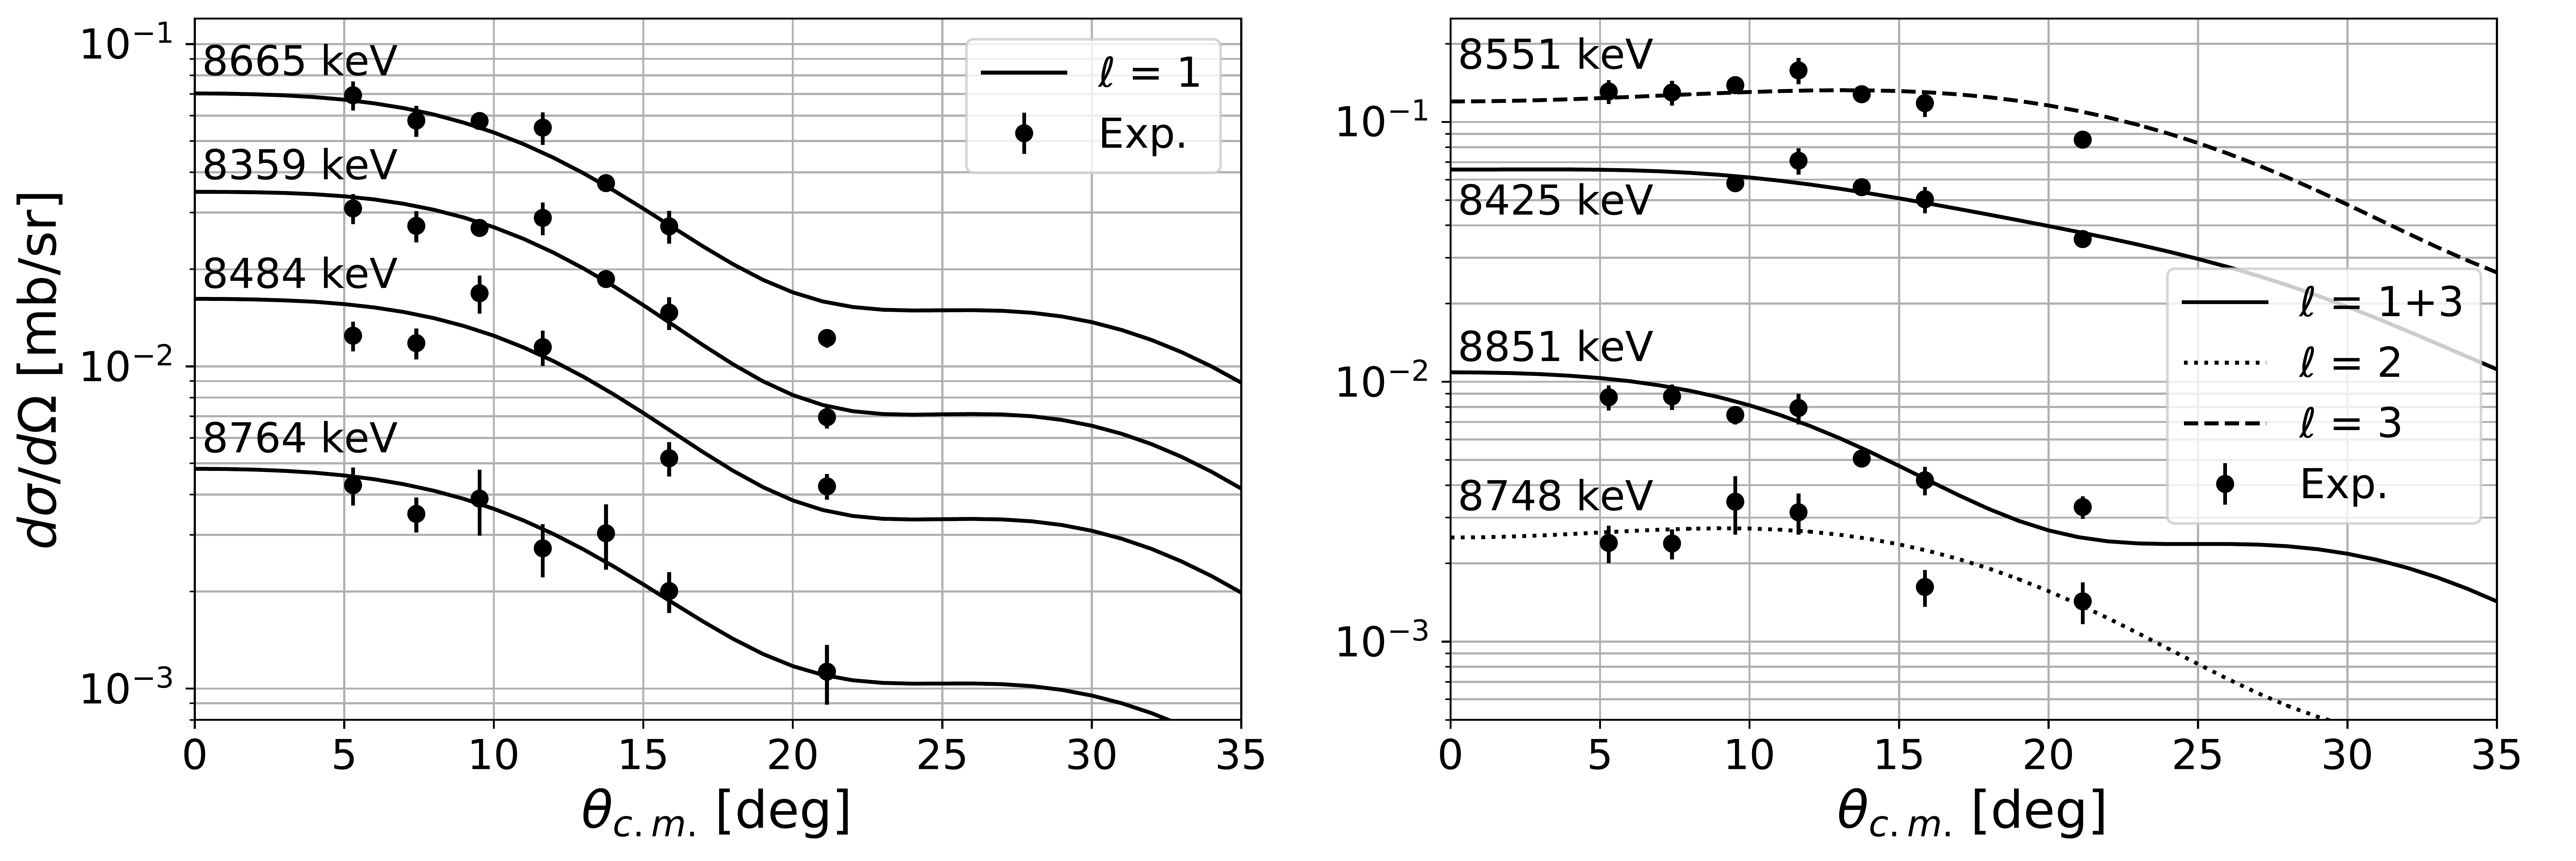
\includegraphics[width=6.5in]{Chapter-6/figs/unbound.png}
\caption{\label{fig:unbound_l}Differential cross-sections of unbound $^{40}\mathrm{Ca}$ states below 8935 keV observed in the present experiment. The left panel shows the $l=1$ distributions, while the right panel shows all other distributions. The experimental data were normalized to the Si detector telescope yield, as described in the text, and further scaling for illustration purposes was not necessary. The zero-range DWBA model curves were computed using the nuclear reaction code, \texttt{FRESCO} \cite{Thompson1988,FRESCO}.}
\end{figure*}

\subsection{Oxidized Targets} \label{subsec:oxidized_cs}

% Effects oxidized targets have on the cross-section
% Adding a 10% scatter? Any corrections? Revisit python notebook to see what I did

\subsection{Spectroscopic Factors from DWBA Models}



\subsection{Proton Partial Widths}



%%%%%%%%%%%%%%%%%%%%%%%%%%%%%%%%%%%%%%%%%%%%%%%%%%%%%%%%%%%%%%%%%%%%%%%%%%%%%%%%%%%%%%%%%%%%%
\section{New $^{39}\mathrm{K}(p,\gamma)^{40}\mathrm{Ca}$ Reaction Rate}

The Monte Carlo reaction rate code, \texttt{RatesMC} \cite{Longland2010a,RatesMC}, was used to calculate a new $^{39}\mathrm{K}(p, \gamma)^{40}\mathrm{Ca}$ reaction rate probability density from the partial-widths and resonance energies reported in this work. Among the states observed in this experiment, only those that do not already have a directly measured resonance strength from $^{39}\mathrm{K}(p, \gamma)^{40}\mathrm{Ca}$ \cite{Kikstra1990,Cheng1981,Leenhouts1966}, i.e. only those below $E_{x} = 8935$ keV, were modified from the most recent reaction rate evaluation of Ref. \cite{Longland2018}. 
%To consolidate the directly measured resonance strengths from Refs. \cite{Kikstra1990,Cheng1981,Leenhouts1966}, we adopt the parameters of Ref. \cite{Longland2018} to obtain the expectation value and variance of these measurements. % Is this okay to say, or should I just say we adopt the expectation values and variances of those measures from Ref. \cite{Longland2018}, not the method itself?
The new reaction rate is compared with that of Ref. \cite{Longland2018} in Fig. \ref{fig:rateCompare}. The solid line and blue band represent the median, recommended rate and the $1\sigma$ confidence interval of this work, respectively. The dotted line and gray band represent that of Ref. \cite{Longland2018}, except with resonance energies calculated using $S_{p} = 8328.18(2)$ keV from Ref. \cite{Wang2021} for consistency, but with marginal effect. Both reaction rates are normalized to the median, recommended rate of Ref. \cite{Longland2018}. %,where the bands represent the 1$\sigma$ confidence interval of each Monte Carlo calculation. 

As mentioned previously, the large uncertainty in Ref. \cite{Longland2018}, between about 50 MK and 200 MK, corresponds to most of the relevant temperatures that reproduce the Mg--K anticorrelation in the globular cluster NGC 2419 \cite{Iliadis2016}. 
%Above 20 MK, the region with the largest uncertainty in Ref. \cite{Longland2018}, between about 50 MK and 200 MK, corresponds to most of the relevant temperatures that reproduce the Mg--K anticorrelation in the globular cluster NGC 2419 \cite{Iliadis2016}.
Fig. \ref{fig:rateCompare} illustrates that the new reaction rate increases significantly in this range, particularly at 70 MK where the median rate is a factor of 13 larger than the rate of Ref. \cite{Longland2018}. The $1\sigma$ width is also significantly reduced in this region, from a factor of 84 at 80 MK to just a factor of 2, a reduction of a factor of 42.

Our new determination of $(2J+1)\Gamma_{p}$ for the 154 keV resonance is primarily responsible for the increase in the rate and decrease in the uncertainty between about 55 MK and 110 MK. Similar effects occur between about 20 MK and 55 MK, primarily from our $l=1+3$ assignment of the 96 keV resonance, which has replaced the $l=3$ assignment by the other $(^{3}\mathrm{He}, d)$ measurements in this calculation. The $(d,n)$ measurement of Ref. \cite{Fuchs1969} is in agreement with the $l=1+3$ assignment for this resonance. Note that using the previous $l=3$ assignment has a negligible effect on the results mentioned above at 70 and 80 MK. Our $(2J+1)\Gamma_{p}$ determination for the 29 keV resonance is responsible for the rate increase below 20 MK. The smaller effects above 110 MK are from a combination of the 335 keV, 415 keV, 439 keV, and 521 keV resonances, the latter three of which have replaced $(2J+1)\Gamma_{p}$ upper limits in Ref. \cite{Longland2018}.

\begin{figure}[t]
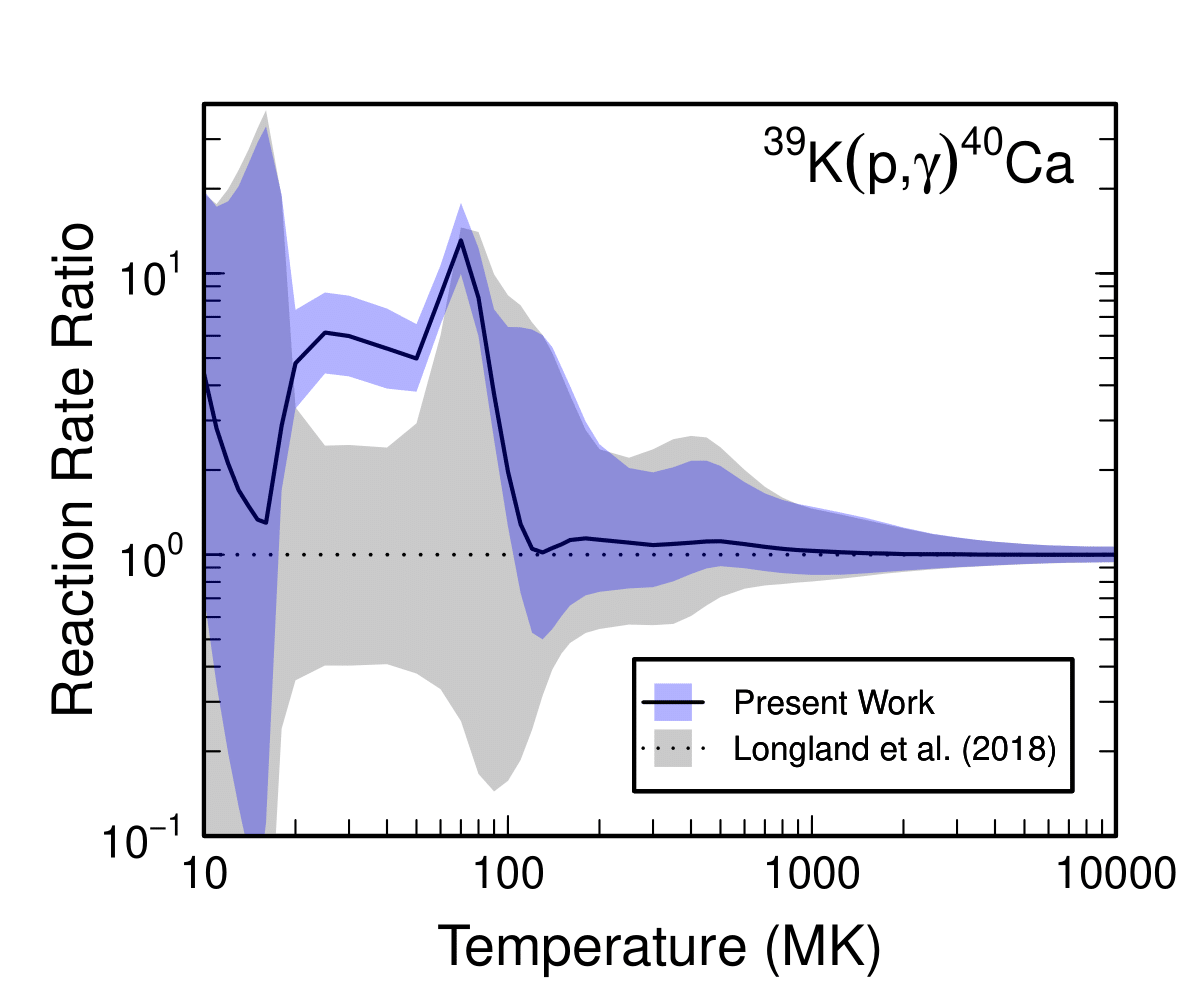
\includegraphics[width=6.5in]{Chapter-6/figs/rateCompare.png} % 6.5 in is exact page width (8.5 in) minus the 1 in margins. Height scaled automatically to keep aspect ratio.
\caption{\label{fig:rateCompare}Comparison between the $^{39}\mathrm{K}(p, \gamma)^{40}\mathrm{Ca}$ reaction rate using the proton partial-widths and resonance energies of the present experiment (solid line, blue band) and the most recent evaluation of Ref. \cite{Longland2018} (dotted line, gray band). The reaction rate ratio is taken with respect to the median, recommended rate of Ref. \cite{Longland2018} for both calculations. The $1\sigma$ uncertainty bands are shown.}
\end{figure}

\begin{figure}[t]
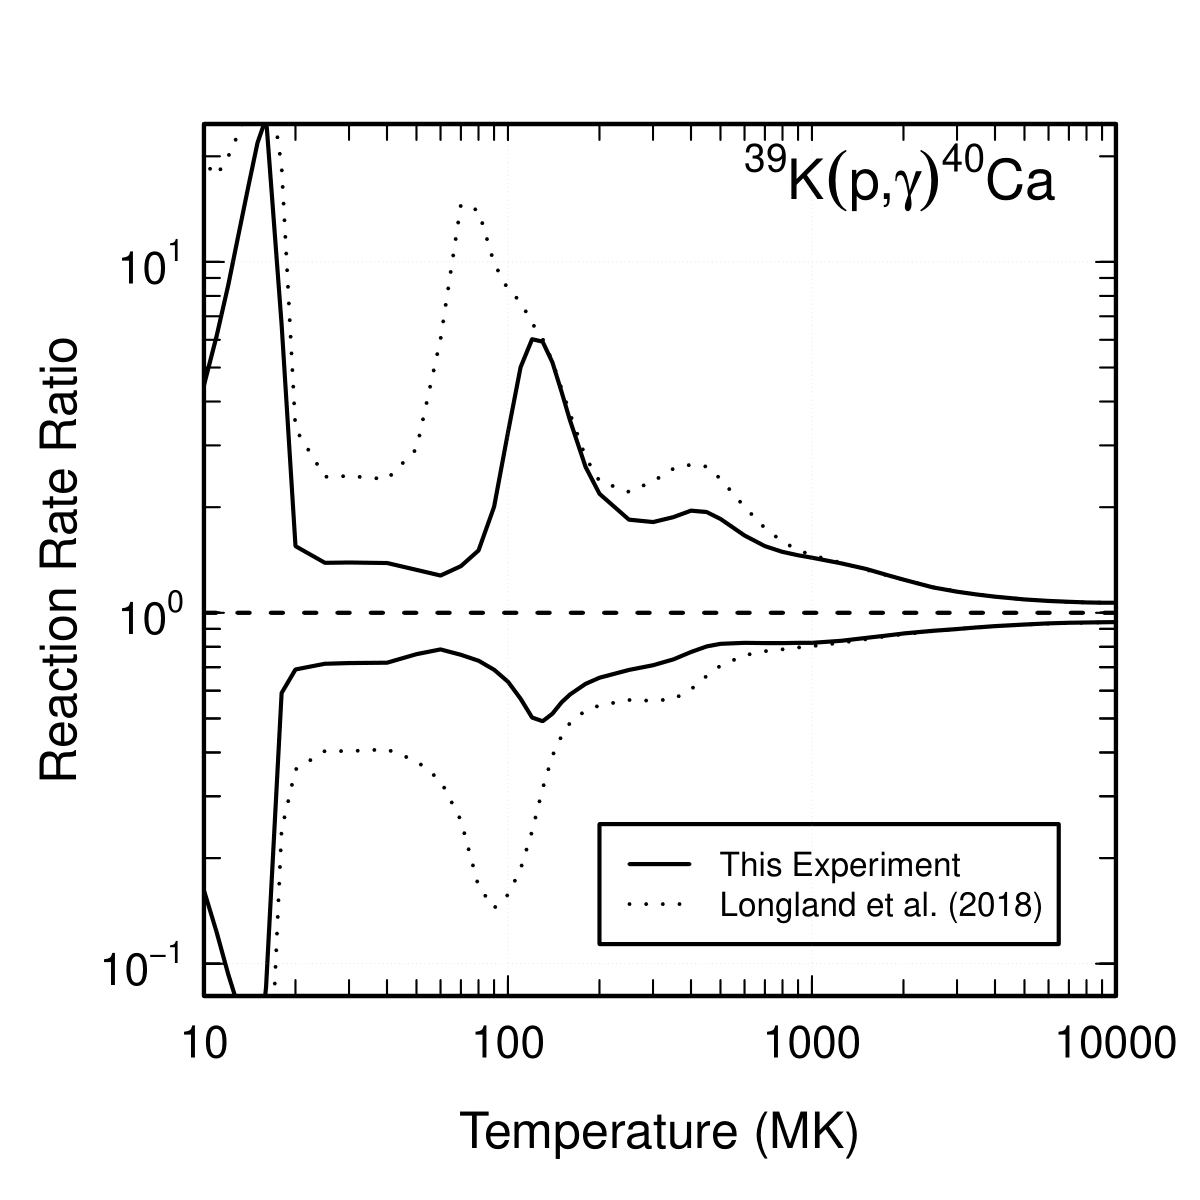
\includegraphics[width=6.5in]{Chapter-6/figs/uncCompare.png} % 6.5 in is exact page width (8.5 in) minus the 1 in margins. Height scaled automatically to keep aspect ratio.
\caption{\label{fig:uncCompare}Comparison between the $^{39}\mathrm{K}(p, \gamma)^{40}\mathrm{Ca}$ reaction rate uncertainty using the proton partial-widths and resonance energies of the present experiment (solid band) and the most recent evaluation of Ref. \cite{Longland2018} (dotted band). Each reaction rate ratio is taken with respect to their own median, recommended rate. The $1\sigma$ uncertainty bands are shown.}
\end{figure}

\begin{figure}[t]
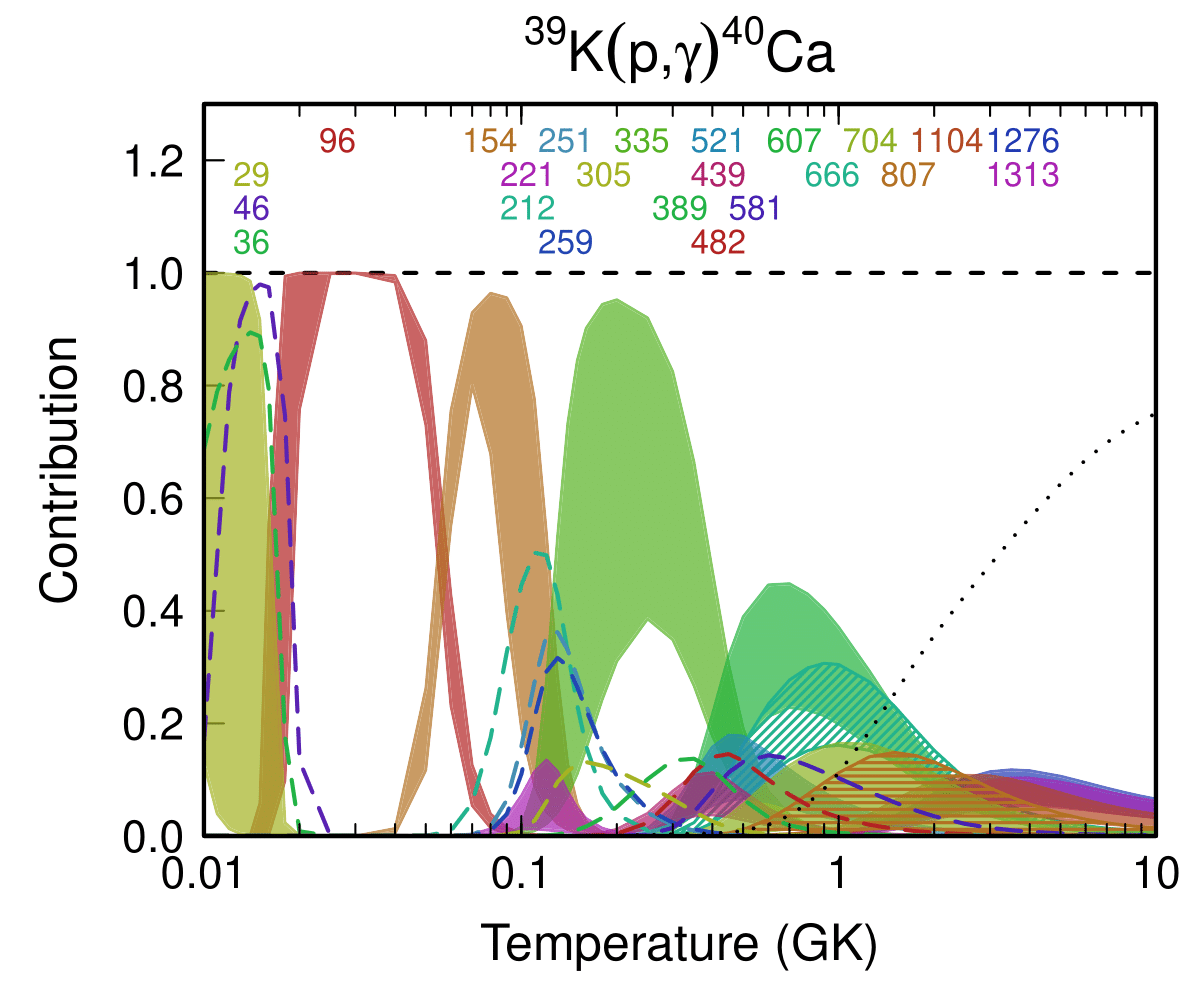
\includegraphics[width=6.5in]{Chapter-6/figs/contrib.png} % 6.5 in is exact page width (8.5 in) minus the 1 in margins. Height scaled automatically to keep aspect ratio.
\caption{\label{fig:contrib}Individual resonance contributions to the $^{39}\mathrm{K}(p,\gamma)^{40}\mathrm{Ca}$ reaction rate, where a value of 1.0 implies that the given resonance contributes 100$\%$ to the reaction rate at that temperature. The labels correspond to the energy of each resonance in keV. Resonances with shading or hatched lines have been measured and are shown with their $1\sigma$ uncertainty bands. Resonances with a single, dashed line are upper limit calculations and show their 84$\%$ "upper" $1\sigma$ value. The resonances displayed are those that individually account for at least 10$\%$ of the total reaction rate at their maximum. The remaining summed resonance contributions are represented by the dotted line.}
\end{figure}

%%%%%%%%%%%%%%%%%%%%%%%%%%%%%%%%%%%%%%%%%%%%%%%%%%%%%%%%%%%%%%%%%%%%%%%%%%%%%%%%%%%%%%%%%%%%%
\section{Potassium Abundance in Reaction Network Calculations}


%%%%%%%%%%%%%%%%%%%%%%%%%%%%%%%%%%%%%%%%%%%%%%%%%%%%%%%%%%%%%%%%%%%%%%%%%%%%%%%%%%%%%%%%%%%%%
\section{Conclusions}


%%%%%%%%%%%%%%%%%%%%%%%%%%%%%%%%%%%%%%%%%%%%%%%%%%%%%%%%%%%%%%%%%%%%%%%%%%%%%%%%%%%%%%%%%%%%%
